\chapter{Experiments}
\label{chapter:experiments}

This chapter aims to describe the experiments in terms of reproducible steps, settings, parameters, conditions, as well as present and discuss results. The ultimate goal is to create an approach for the first task of the ISIC 2019 challenge in such a way that conclusions can be drawn from it. \par


Several important aspects were identified and talked about in \autoref{chapter:sota} that are essential for such an approach. Therefore, this chapter is divided into 5 different sections which hopefully addresses each of those aspects in a systematic way. \par

First, \autoref{section:models} will study which pre-trained models work best for this classification task and the overall impact of transfer learning and neural network architectures in problems like these. Next, \autoref{section:hyperparameters} will methodically optimize the chosen model's hyperparameters through common reasoning to hopefully improve performance and draw conclusions from it. This will be followed by \autoref{section:balance} which will address different methods of dealing with unbalanced data and discuss the importance behind such task. Then, \autoref{section:ensemble} will improve the approach's performance by finding a suitable way for ensembling multiple models. Finally, \autoref{section:outdist} dealing with out of distribution through different procedures. \par 

\section{Pre-trained model choice} \label{section:models}
    In order to classify skin lesions through deep neural networks two approaches can be taken. The first is to create a model from scratch, design it's architecture and train it from the ground up. However, this approach is troublesome because it requires reasoning, setting many hyperparameters simultaneously and cross-validating a wide range of values which is computationally expensive. Another approach is through the use of transfer learning by leveraging the weights of pre-trained models. This is a good option when data is scarce, which is often the case of computer vision related problems. Additionally, there is a wide range of pre-trained models to chose because of challenges such as such as the ILSVRC. \par
    
    In \ref{chapter:sota} several pre-trained models were shown such as ResNet, DenseNet, VGGNet and EfficientNet. All of these were pre-trained on ImageNet with millions of samples of photos of categories such as dogs or cats. As it stands, these models can be re-purposed for skin lesion classification through transfer learning, which was the most common approach to the ISIC 2019. \par
    The first step is to filter which pre-trained models should be considered for the problem of skin lesion classification. For our study we consider commonly used pre-trained models from skin lesion classifiers presented in \autoref{chapter:sota}, which are readily available through the tf.keras.applications framework. More specifically, different variations from the VGG, ResNet, DenseNet, Inception and EfficientNet pre-trained models were considered. Each of these have their own architectural principles and design concepts, and their corresponding variations are based on a baseline model which is scaled up and down. \par
    A benchmark has been set in order to provide a fair evaluation for each of these models:
    \begin{itemize}
        \item Each model is trained on a undersampled version (4000 training samples and 1000 validation samples) of the ISIC 2019 dataset that maintains the original class distribution. The undersampling process is done by randomly picking samples from the original dataset in a stratified manner. This smaller dataset will substantially decrease each model train time, which will allow us to train more pre-trained models in a agile manner. Presumably, a undersampled version of the original dataset will yield similar results as if the whole dataset was being used. 
        \item All image samples are standarized relative to the ISIC 2019 dataset mean RGB channel values.
        \item Extracting all layer's weights while also fine-tuning these layers, which presumably yields higher performance since it will continue to optimize parameters relative to the target dataset, thus minimizing error on said dataset and generalizing well to similar test data. Several other approaches were also tried such as only fine tuning from the middle layer to the top of the network (i.e.) or freezing all the network and only training the classifier. However, both had considerably worse performance, and possibly required a more comprehensive study like the one done in \cite{maia} for each of the pre-trained models which would be troublesome.
        \item The top layer from each pre-trained model is removed and replaced by a global average pooling layer to reduce the number of parameters before the classifier. 
        \item The classifier is composed of one layer of 512 neurons which are fully connected, and each neuron uses the ReLU activation function and one softmax layer with 8 neurons to translate each of the class's probabilities. Meaning that the model classification is given by the softmax value which is the highest. In Figure \ref{fig:softmax_examples} one can see 3 examples of samples taken from ISIC 2019 dataset being classified into probabilities by one of the models.
        \item Online data augmentation is performed with random crops, flips, rotations, shears, brightness changes and color changes, in order to minimize overfitting while training.
        \item All image samples are resized before passing through the network to each pre-trained models input size. All the presented pre-trained models have a square input aspect ratio, so no image distortions happen while resizing.
        \item The following the work done by \cite{gessert2018} the Adam optimizer is used, with a categorical cross entropy loss function. 
        \item A batch size of 32 is used with a learning rate of 0.0001. However, the learning rate is reduced by a factor of 0.1 when validation loss stops improving for 8 epochs.
        \item Train for a maximum of 100 epochs. However, early stopping is performed whenever validation loss stops improving for 16 epochs.
        \item For each training process 3 models are saved. The model up to a certain epoch that obtained the highest balanced multi-class accuracy on the validation set, the model up to a certain epoch that obtained the lowest loss on the validation set, and finally the latest model from the last epoch. It is hypothesized that the latest model will have worse generalization than that of the other 2 models. 
    \end{itemize}
    
    \begin{figure}[ht]
        \centering
        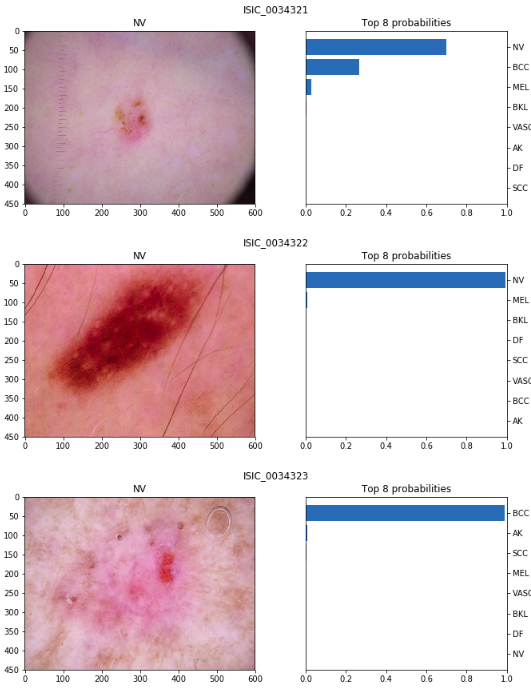
\includegraphics[scale=1.5, width=\textwidth]{figs/softmax_examples.png}
        \caption{3 Softmax probabilities created from 3 samples of the ISIC 2019 dataset}
        \label{fig:softmax_examples}
    \end{figure}
    
    The simplest way of re-purposing a pre-trained model is by only replacing it's classifier. For this procedure, the top layers of the pre-trained model must be removed, which are the layers that are not convolutional or pooling layers at the end of the pre-trained model's architecture, and the weights from the trainable layers of the convolutional base must be freezed, by setting their trainable property to false. Figure \ref{fig:pre_trained_models_classifier_comp} compares the results of applying this approach to several pre-trained models in terms of test accuracy and test balanced multi-class accuracy. One can see that the overall performance is bad, with the best architectures being VGG and EfficientNet. These results are to be expected because the weights of the layers of the convolutional base of these models were all trained to a very different dataset (ImageNet), from the one we are now trying to re-purpose the model to (ISIC 2019 dataset).  \par
    \begin{figure}[ht]
        \centering
        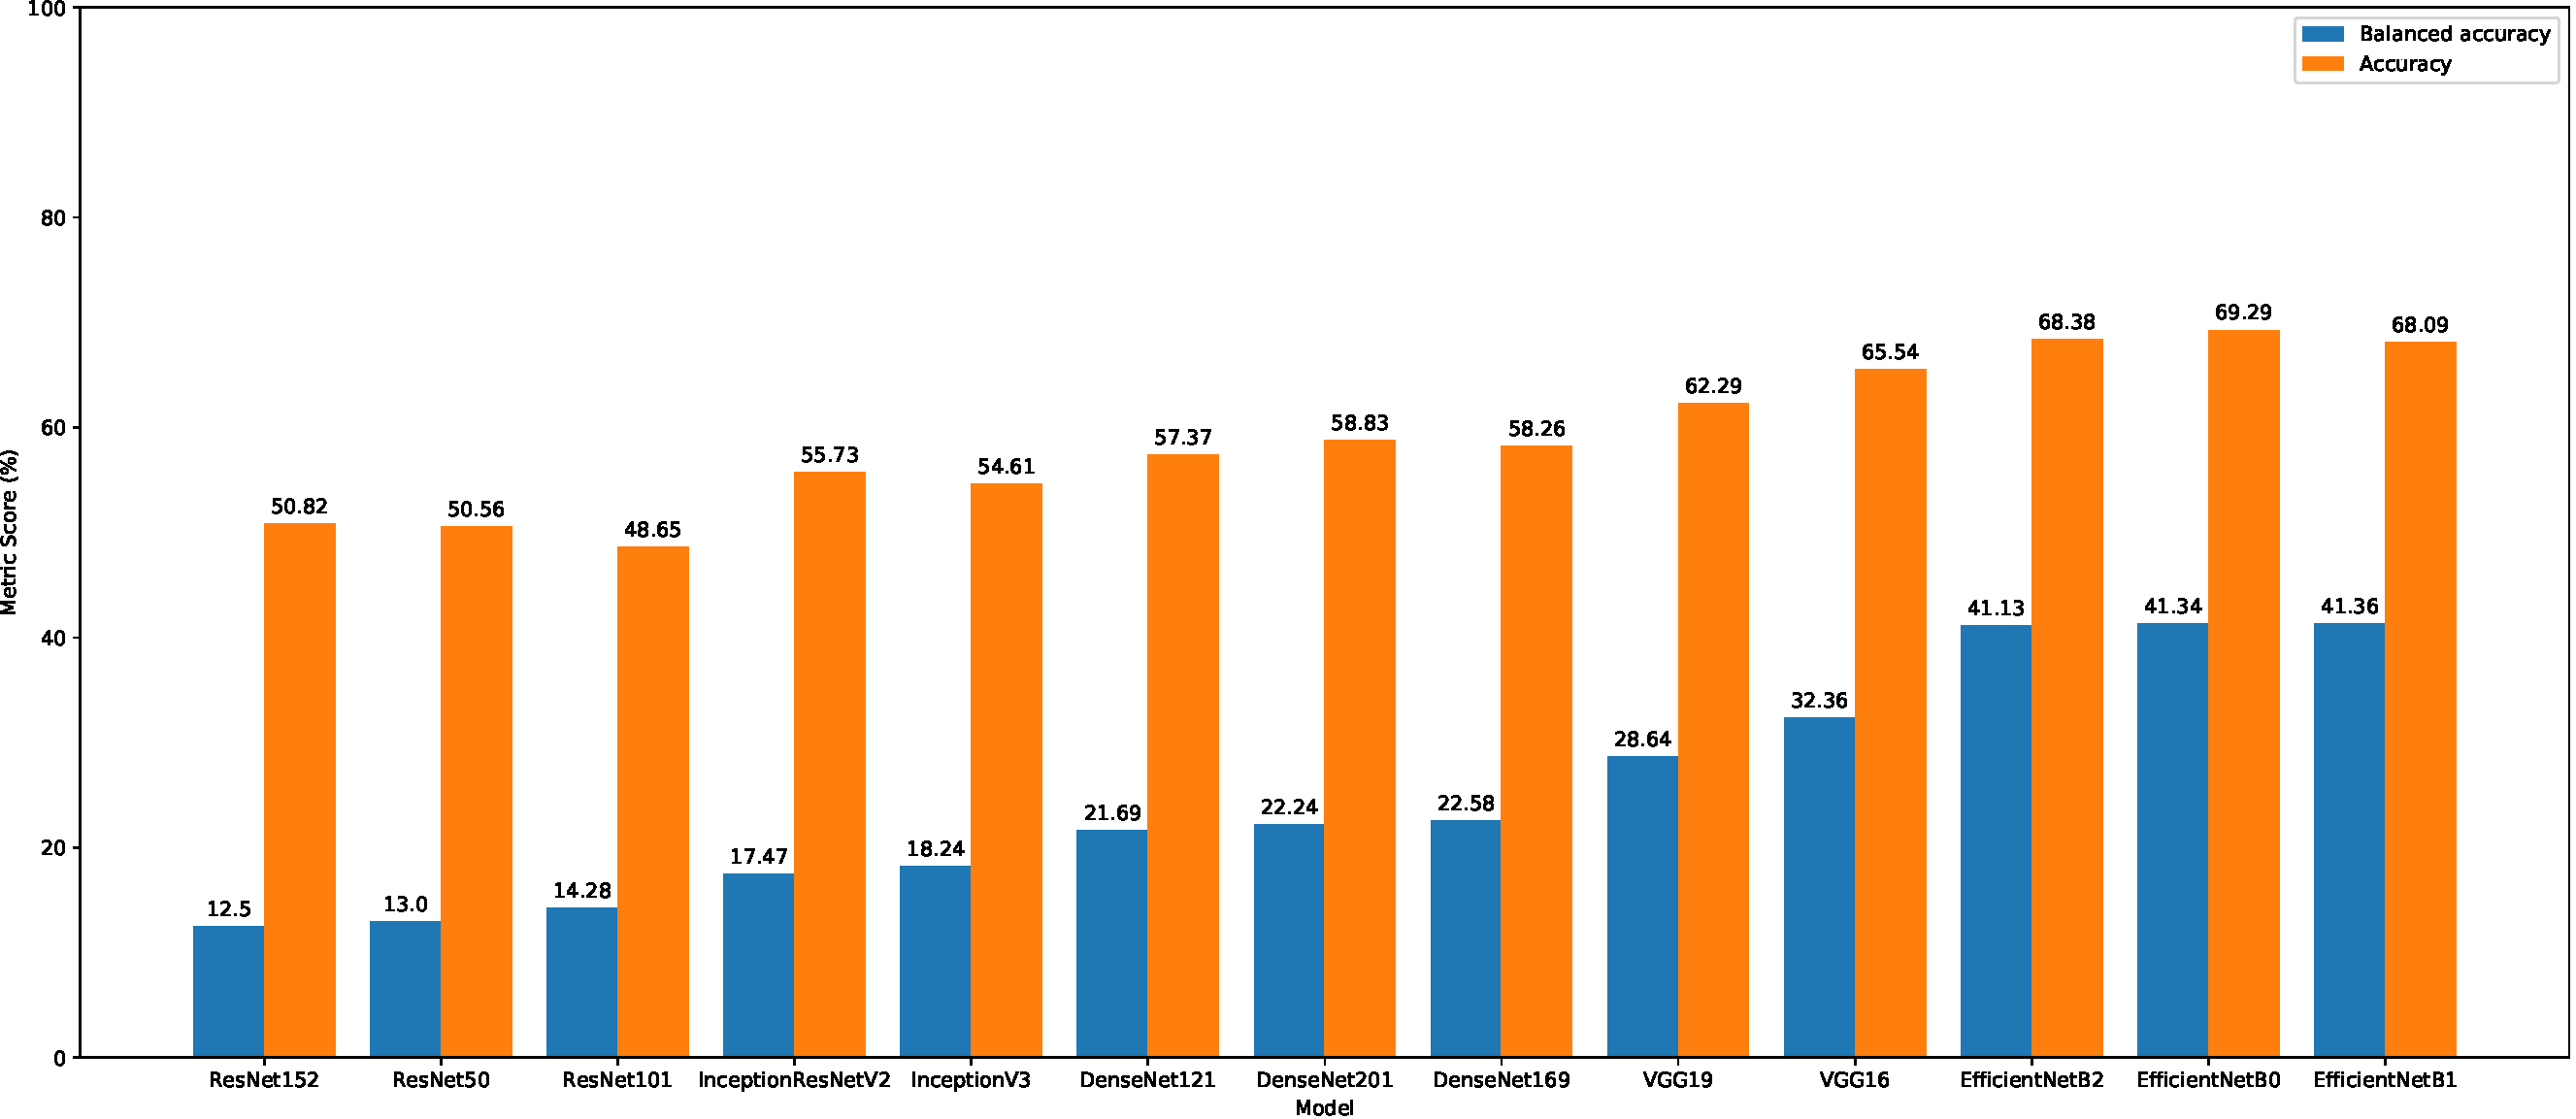
\includegraphics[scale=1.5, width=\textwidth]{figs/pre_trained_models_classifier_comp.pdf}
        \caption{Balanced multi-class accuracy and accuracy of various pre-trained models by replacing the top layers (classifier)}
        \label{fig:pre_trained_models_classifier_comp}
    \end{figure}
    
    Therefore, a more sensible approach to this problem is to adapt the whole set of parameters to this new dataset while also taking advantage of the already existing weights trained on ImageNet. This approach is based on the fine-tuning concept, meaning that all the weights from the pre-trained model are transferred to the new model, but are also updated along with the classifier on each epoch. Presumably, by taking this approach, the knowledge obtained from the existing weights will be adapted to a new problem and increase performance results on the test set. Figure \ref{fig:pre_trained_model_val_comp} shows that this assumption is true, as all pre-trained model's had a significant increase in both accuracy and balanced multi-class accuracy when compared with \ref{fig:pre_trained_models_classifier_comp}.  \par
    \begin{figure}[ht]
        \centering
        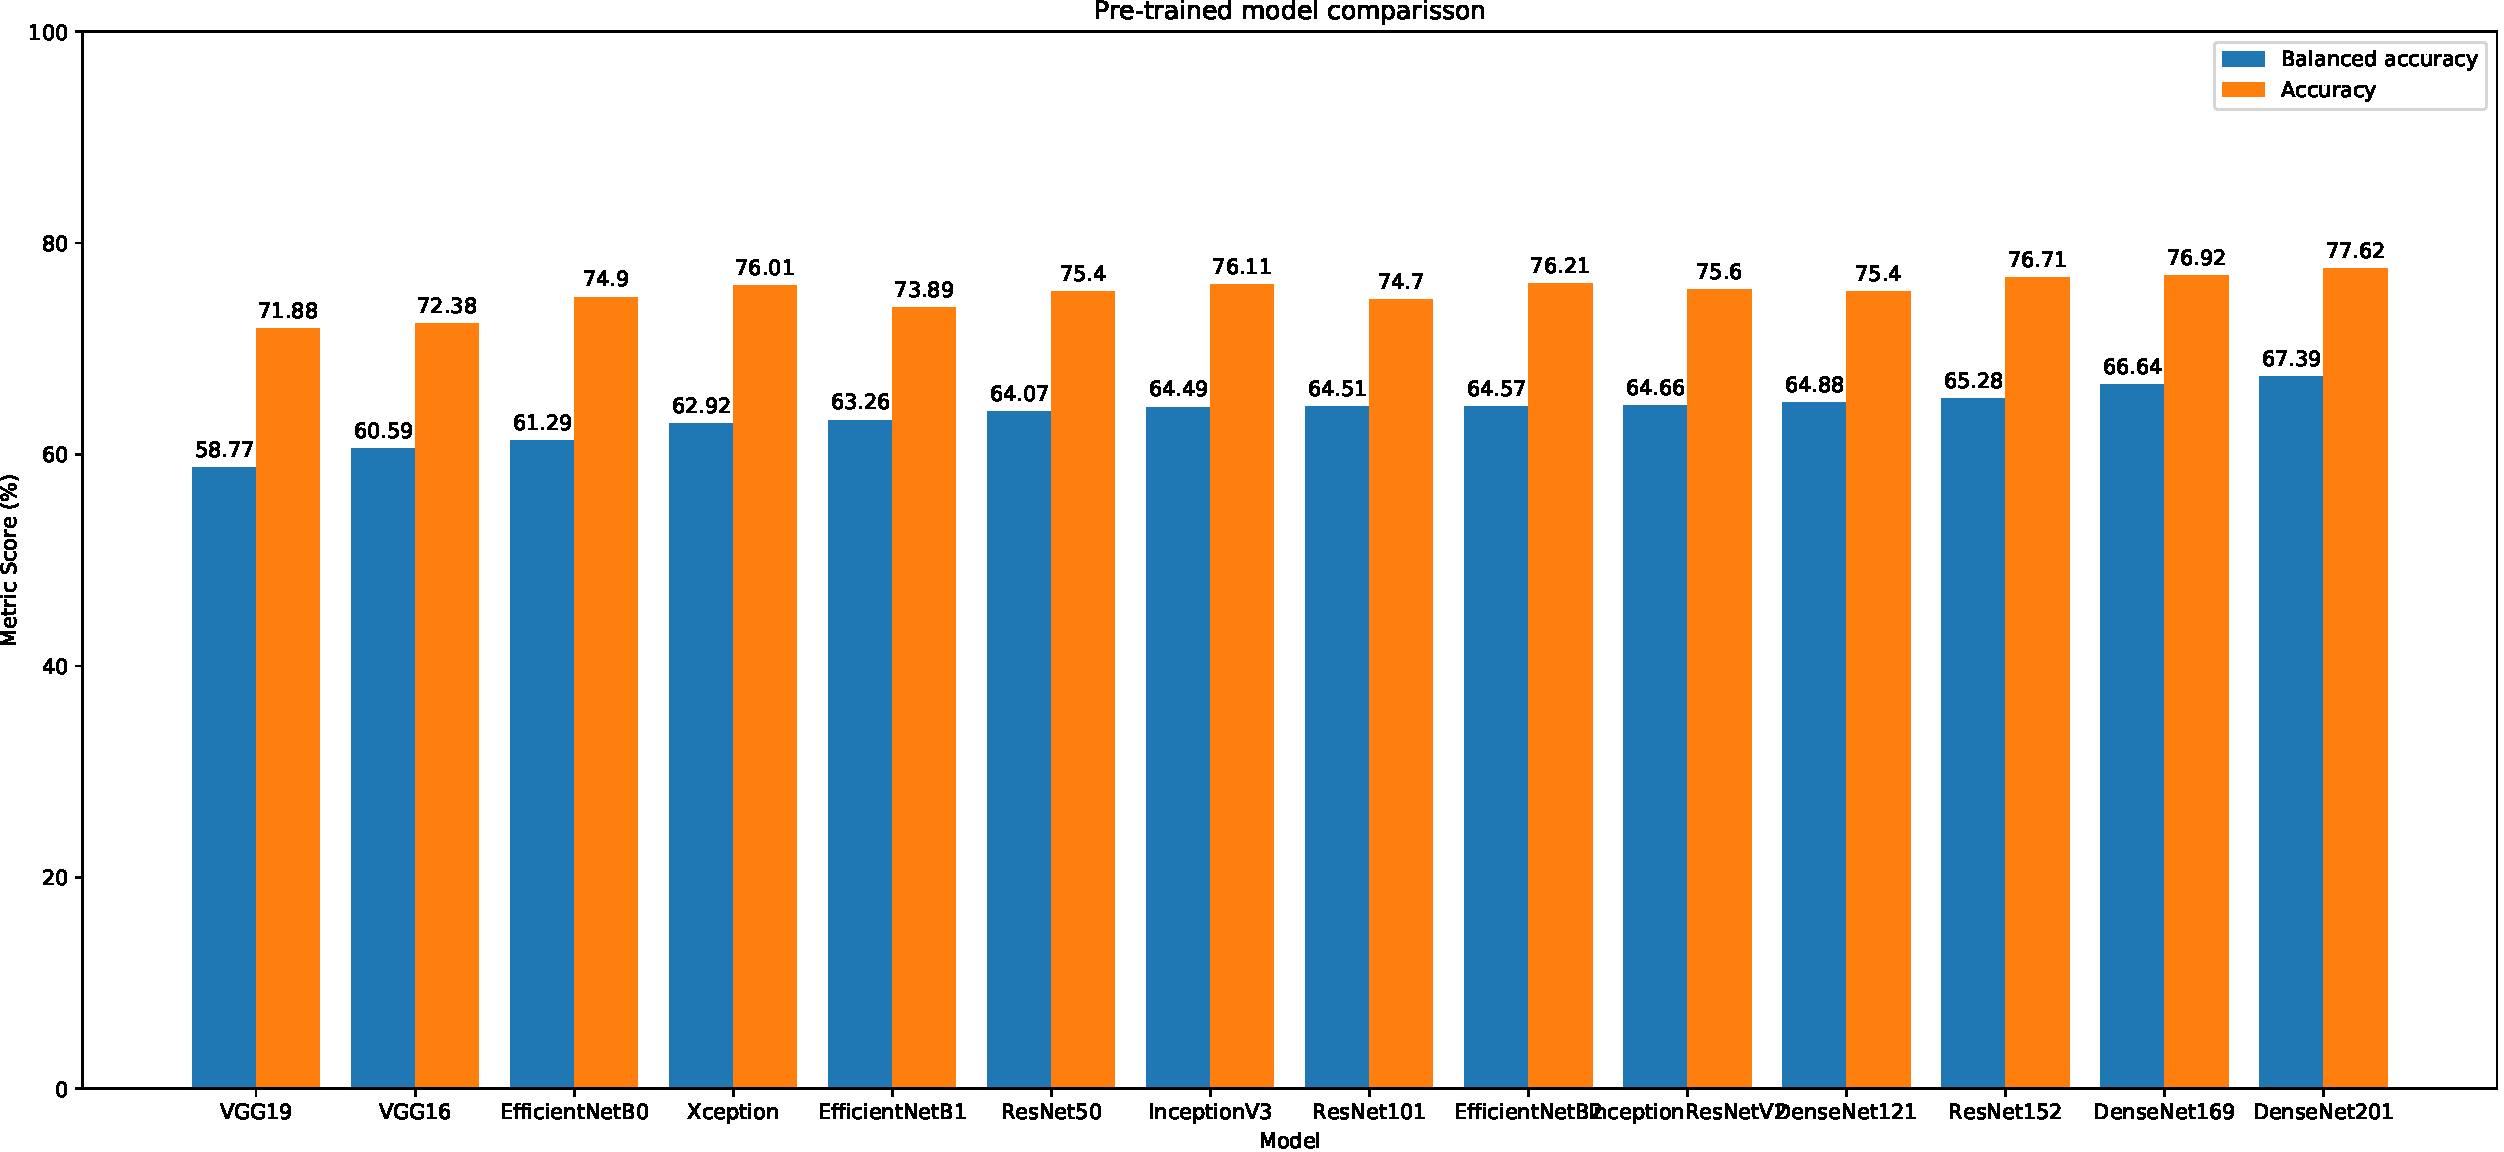
\includegraphics[scale=1.5, width=\textwidth]{figs/pre_trained_models_val_comp.pdf}
        \caption{Balanced multi-class accuracy and accuracy of various pre-trained models on fine tuning the whole model and replacing the top layers(classifier)}
        \label{fig:pre_trained_model_val_comp}
    \end{figure}
    
    In general, one can see that the balanced model accuracy is much lower than the accuracy in every trained model. That is due to the fact that the data is imbalanced and more true predictions are made towards classes with higher number of samples (illustrated in Figure \ref{fig:densenet201_pred_dist}), which the accuracy metric does not take into account. On the other hand the balanced multi-class accuracy is the mean recall of each class and therefore the performance of the model in each class is weighted the same, which substantially lowers the values. \par
    \begin{figure}[ht]
        \centering
        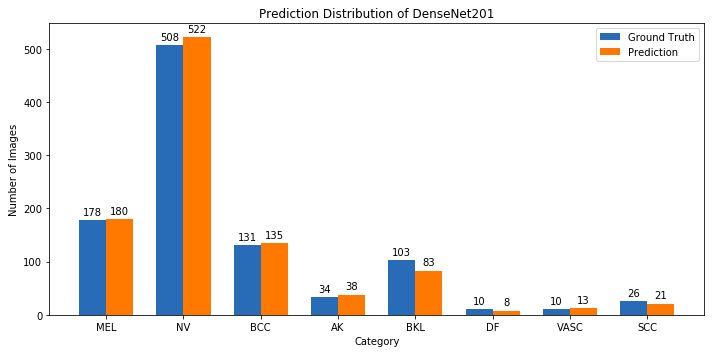
\includegraphics[width=\textwidth]{figs/densenet201_pred_dist.png}
        \caption{Prediction distribution of DenseNet201}
        \label{fig:densenet201_pred_dist}
    \end{figure}
    
    Generally, by looking at Table \ref{tables:pretrainedmodels} we can see that more recent architectures such as DenseNet or Inception perform better than older architectures such as VGG. This can be attributed to the fact that the VGG16 and the VGG19 are shallower models compared to the others. It is to be expected that deeper models have a positive impact on model accuracy, because more layers have the ability to create more levels of abstraction. To put this into test we compared for each "family" of architectures the influence of depth on model accuracy. \par 
    
    The one exception to the depth rule is presented by the VGG family of models, which does not improve performance with depth increase (Illustrated in \ref{fig:vgg_depth}). In fact, VGG19 also performed worse than VGG16 on the ILRSVC challenge as shown in \ref{tables:pretrainedmodels}. We presume this is related to the vanishing gradients problem, which typically becomes a larger concern for deeper networks because the gradient decreases exponentially as we propagate down to the initial layers \cite{Nielsen2017a}. \par 
    \begin{figure}[ht]
        \centering
        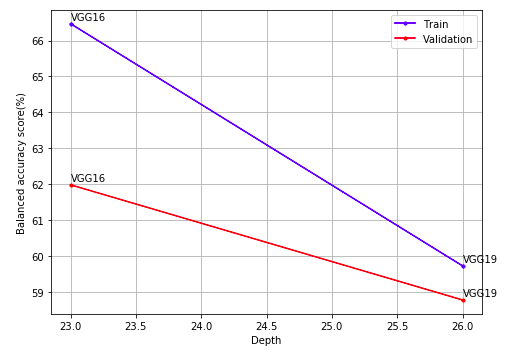
\includegraphics[width=0.7\textwidth]{figs/vgg_depth.png}
        \caption{Influence of depth on VGG pre-trained models}
        \label{fig:vgg_depth}
    \end{figure}
    
    This problem was later addressed by architectures such as ResNet, which would allow it to build models up to 152 layers deep. In this study we will compare ResNet50, ResNet101 and ResNet152 with 50, 101 and 152 depths, respectively. We can see the impact of model depth on ResNet performance in \ref{fig:resnet_depth}, which shows that model depth is directly correlated to validation balanced accuracy in a linear way for this specific architecture. He et al \cite{resnet} tried to go further and created a ResNet1202 layer deep network, but it performed worse than the 152 version, which it was resolved as an overfitting problem due to a large number of parameters for the size of the given dataset, showing the disadvantages of models which are too large.  \par
    \begin{figure}[ht]
        \centering
        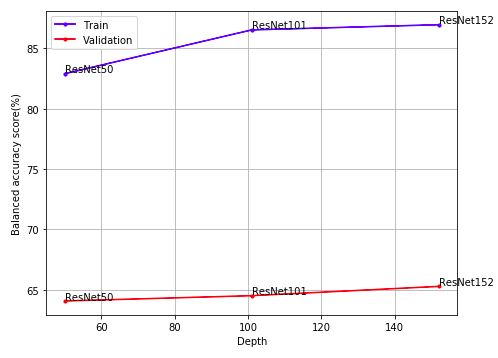
\includegraphics[width=0.7\textwidth]{figs/resnet_depth.png}
        \caption{Influence of depth on ResNet pre-trained models}
        \label{fig:resnet_depth}
    \end{figure}
    DenseNet also extended the idea further which would allow it to build even deeper models, namely with 121, 169 and 201 layers. It should also be noted that there is a 264 version of this network, however as it was not available for the tf.keras framework it was discarded. One can can see how depth impacts the validation performance of the DenseNet architecture on \ref{fig:densenet_depth}. Surprisingly, DenseNet201 has the worst performance on the training set, however it also has the highest BMA, contrarily to DenseNet169 which is overfitting due to the huge disparity between training BMA and validation BMA. \par
    \begin{figure}[ht]
        \centering
        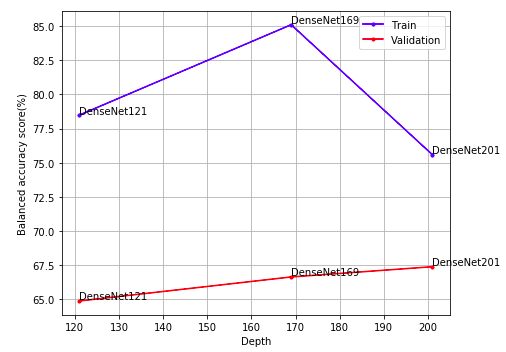
\includegraphics[width=0.7\textwidth]{figs/densenet_depth.png}
        \caption{Influence of depth on DenseNet pre-trained models}
        \label{fig:densenet_depth}
    \end{figure}
    
    Even though within the same architecture deeper models tend to perform better, the increased depth means more trainable parameters which means that the requirements for memory and processing power increase. An inefficient use of model parameters might lead to overfitting because the network can tune them to a very specific set of data \cite{?}. EfficientNets address this problem with the compound scaling method presented in \autoref{chapter:sota}, which not only scales depth, but also input input size and layer width. We can see it's effectiveness in \ref{fig:efficientnet_params}.
    \begin{figure}[ht]
        \centering
        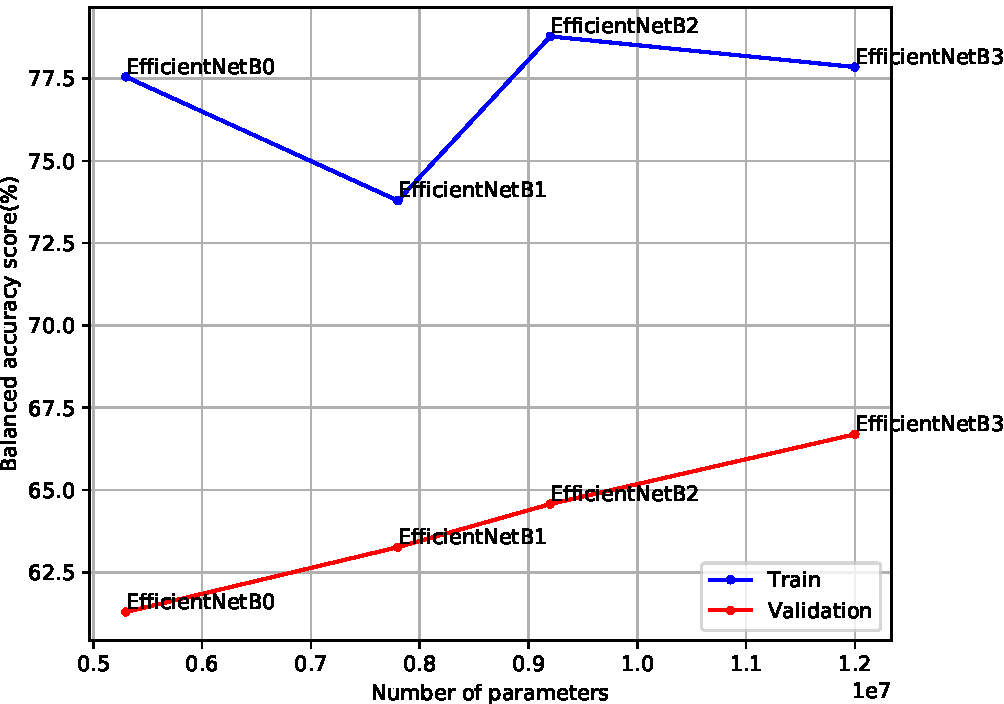
\includegraphics[width=0.7\textwidth]{figs/efficientnet_params.pdf}
        \caption{Influence of model parameters on EfficientNet performance}
        \label{fig:efficientnet_params}
    \end{figure}
    
    As shown in the confusion matrix of Figure \ref{fig:densenet201_untuned_conf_matrix}, even the DenseNet201, which was the best performing model, struggles on classification of underrepresented classes such as vascular lesions, while performing well with overepresented classes such as the melanocytic nevus. Considering the results, more data from underrepresented classes need to be fed into the training process in order to improve classification performance, Nonetheless, this provides the baseline model which should serve as a benchmark comparison in the next sections. \par
    \begin{figure}[ht]
        \centering
        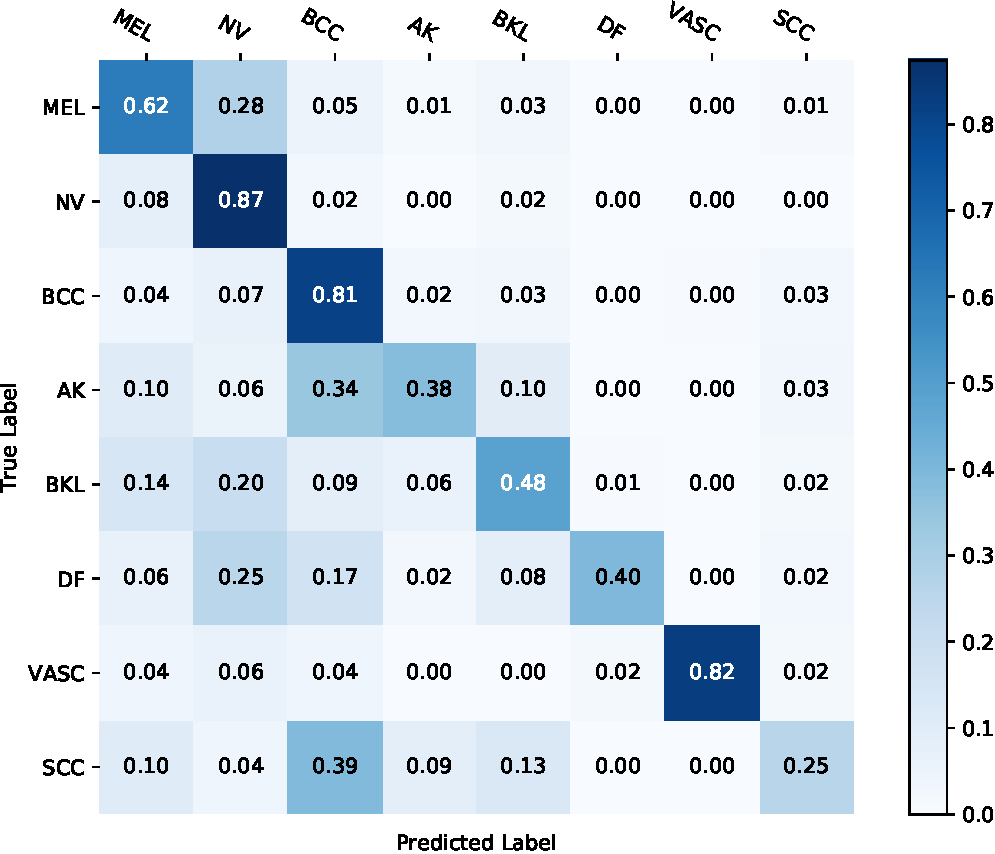
\includegraphics[width=0.6\textwidth]{figs/densenet201_untuned_conf_matrix.pdf}
        \caption{Confusion matrix of the hyperparameter tuned DenseNet201}
        \label{fig:densenet201_untuned_conf_matrix}
    \end{figure}

\section{Hyperparameter optimization} \label{section:hyperparameters}

    In order to achieve the best possible performance using a transfer learning method, pre-trained models need to be hyperparameter tuned to obtain the best possible combination of hyperparameters for the problem at hand.  As such, in order to tune hyperparameters usually the holdout method is applied, meaning that a different set of data (validation set) is used for evaluation to get an unbiased assessment of the model’s generalization performance. The validation set is required because if one uses the test set for this optimization then there is a high risk of optimistically biasing the model \cite{talbot}. Even though the holdout method has it's downsides, we applied it because time requirements are much lower compared to techniques like nested cross validation or k-fold cross validation. \par
    
    In order to systematically find each hyperparameter in an efficient way, the strategy presented in \ref{?} will be used. Additionally, for this evaluation a benchmark has been set in order to compare the results in a fair manner:
    \begin{itemize}
        \item Each model is trained on a undersampled version (4000 training samples and 1000 validation samples) of the ISIC 2019 dataset that maintains the original class distribution. The undersampling process is done by randomly picking samples from the original dataset in a stratified manner. This smaller dataset will substantially decrease each model train time, which will allow us to train more pre-trained models in a agile manner. Presumably, a undersampled version of the original dataset will yield similar results as if the whole dataset was being used. 
        \item All image samples are standarized relative to the ISIC 2019 dataset mean RGB channel values.
        \item Extracting all layer's weights while also fine-tuning these layers, which presumably yields higher performance since it will continue to optimize parameters relative to the target dataset, thus minimizing error on said dataset and generalizing well to similar test data. Several other approaches were also tried such as only fine tuning from the middle layer to the top of the network (i.e.) or freezing all the network and only training the classifier. However, both had considerably worse performance, and possibly required a more comprehensive study like the one done in \cite{maia} for each of the pre-trained models which would be troublesome.
        \item The top layer from each pre-trained model is removed and replaced by a global average pooling layer to reduce the number of parameters before the classifier. 
        \item The classifier is composed of one layer of 512 neurons which are fully connected, and each neuron uses the ReLU activation function and one softmax layer with 8 neurons to translate each of the class's probabilities. Meaning that the model classification is given by the softmax value which is the highest. In Figure \ref{fig:softmax_examples} one can see 3 examples of samples taken from ISIC 2019 dataset being classified into probabilities by one of the models.
        \item Online data augmentation is performed with random crops, flips, rotations, shears, brightness changes and color changes, in order to minimize overfitting while training.
        \item All image samples are resized before passing through the network to each pre-trained models input size. All the presented pre-trained models have a square input aspect ratio, so no image distortions happen while resizing.
        \item For each training process 3 models are saved. The model up to a certain epoch that obtained the highest balanced multi-class accuracy on the validation set, the model up to a certain epoch that obtained the lowest loss on the validation set, and finally the latest model from the last epoch. It is hypothesized that the latest model will have worse generalization than that of the other 2 models. 
    \end{itemize}
    
    One important aspect of training deep neural networks is the number of epochs that it will run on. One epoch is when all training examples have been forward and backward passed through the network. In other words, one epoch means that every image has been seen. Therefore, the number of epochs define how many times each image is seen by the network. We fixed the maximum number of epochs to 100 (even though most of our models never reach close to it). \par
    
    However, we are fine tuning a pre-trained model with a new classifier on top, which means that the classifier's weights are all at 0. We hypothesized that the initial weights of the classifier are determinant for the overall model performance. So in order to deal with this problem for an initial number of epochs we will freeze all the pre-trained model's layers and only tune the classifier weights just to minimize the impact of the initial weights of the network on the overall performance. Figure \ref{fig:wiepochs_comp} illustrates the impact of the number of weight initializing epochs on the overall performance. \par
    \begin{figure}[ht]
        \centering
        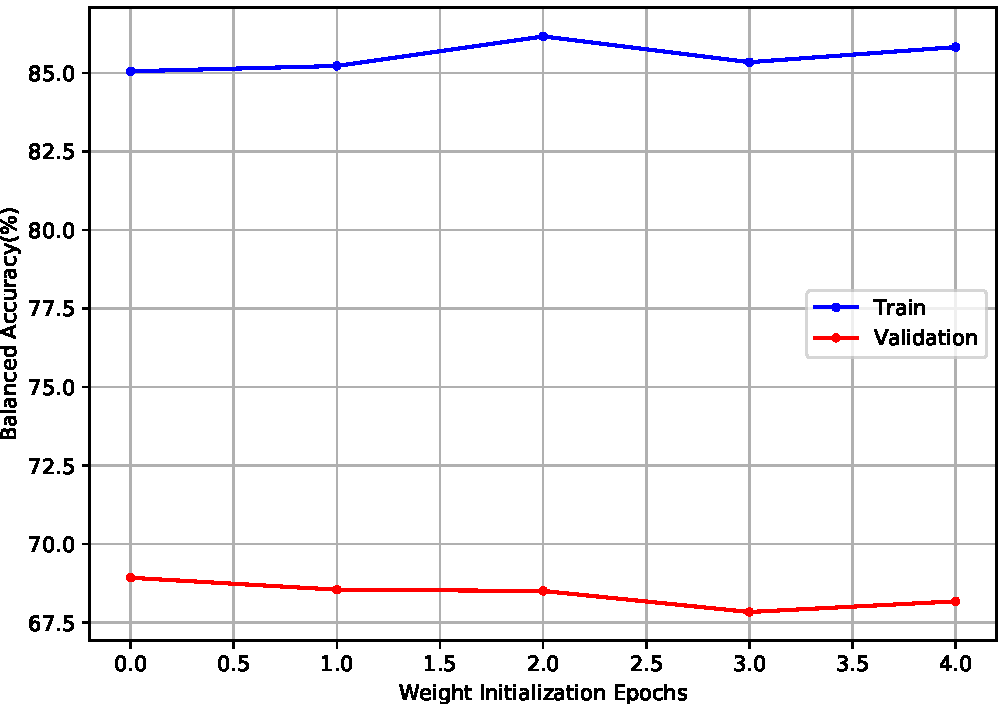
\includegraphics[width=0.6\textwidth]{figs/densenet201_wiepochs_comp.pdf}
        \caption{Influence of weight initialization epochs on train and validation balanced multi-class accuracy}
        \label{fig:wiepochs_comp}
    \end{figure}
    
    Batch size can also be an important factor to consider. It defines the number of training images passed through the network in one forward and backward pass. The bigger the batch size the more memory is needed and the faster the network is going to converge, because there are fewer iterations per epoch. The size is directly correlated to the number of iterations per epoch by equation \ref{eq:iter_epoch}.
        \begin{equation}
        \mbox{iterations per epoch}=\frac{\mbox{training images}}{\mbox{batch size}}
        \label{eq:iter_epoch}
        \end{equation}
    Where one iteration is one backward and forward pass, which means that larger batch sizes will make less iterations per epoch, which means that the model will train faster. \par
    \begin{figure}[ht]
        \centering
        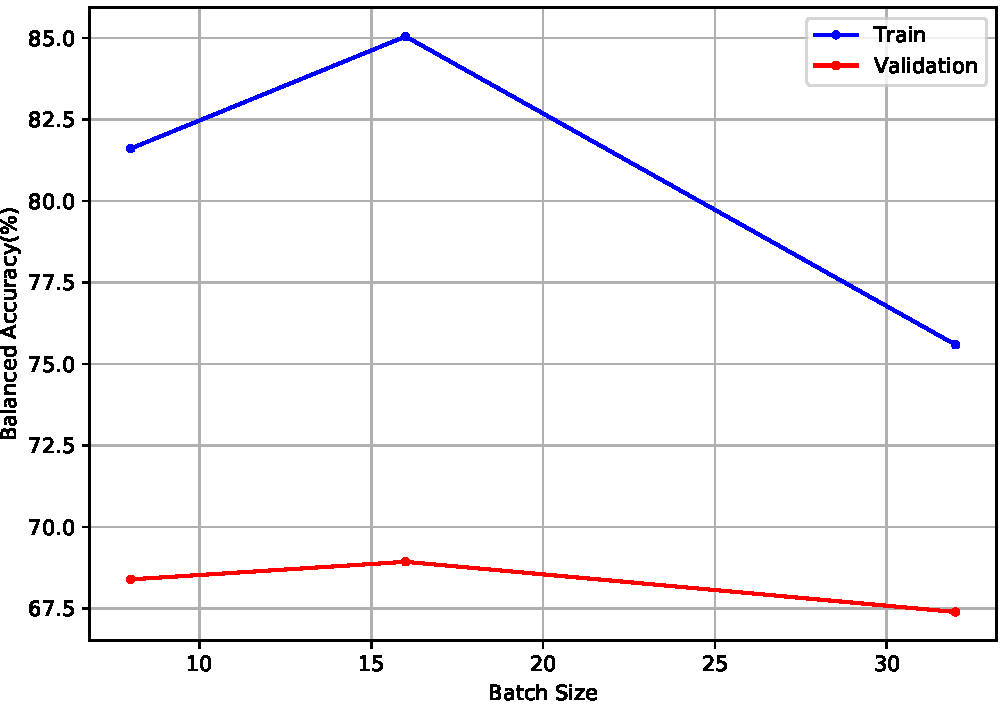
\includegraphics[width=0.6\textwidth]{figs/densenet201_batch_comp.pdf}
        \caption{Influence of batch size on train and validation balanced multi-class accuracy}
        \label{fig:batch_comp}
    \end{figure}
    
    Perhaps the most important hyperparameter to optimize is the learning rate. It controls the step size for model weight updates with respect to the loss function. Lower values mean slower travel along the downward slope, which consequently takes longer times to converge. In this approach, two learning rates are considered. \par 
    
    We vary the learning rate which is used to initialize the weights of the classifier during weight initialization epochs and illustrate the results in figure \ref{fig:wilr_comp}. \par
    \begin{figure}[ht]
        \centering
        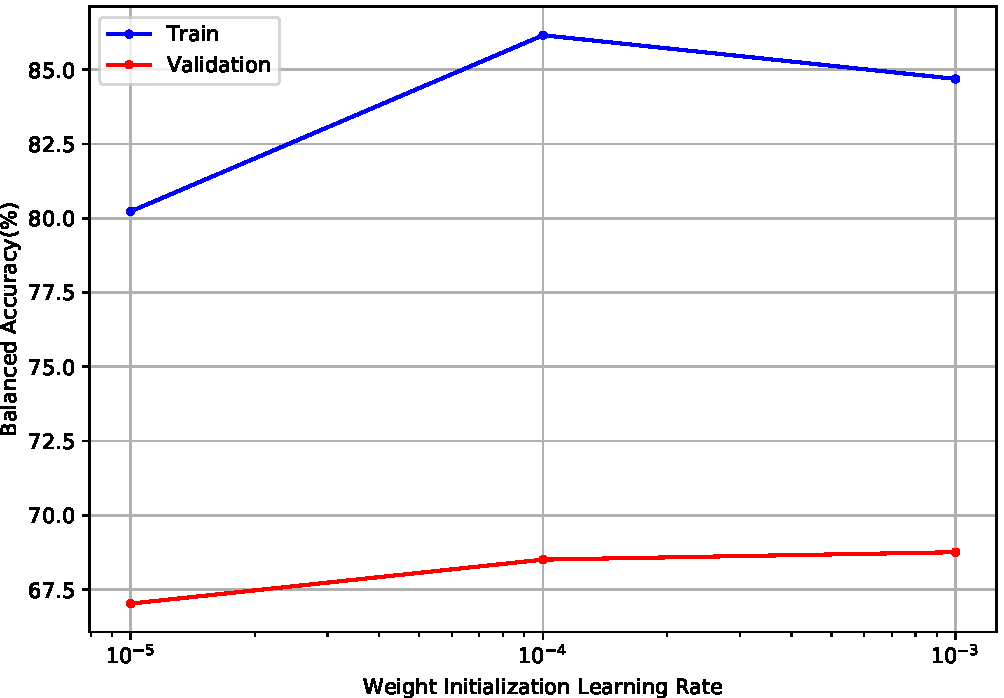
\includegraphics[width=0.6\textwidth]{figs/densenet201_wilr_comp.pdf}
        \caption{Influence of weight initialization learning rate on train and validation balanced multi-class accuracy}
        \label{fig:wilr_comp}
    \end{figure}
    
    Figure \ref{fig:wilr_lr_over_epochs} illustrates the evolution of the learning rate over the epochs for different weight initialization learning rates. One can see the lower learning rates make the model to converge later and specifically with a learning rate of $1e-5$ the model converges to a local minimum earlier on. \par
    \begin{figure}[ht]
        \centering
        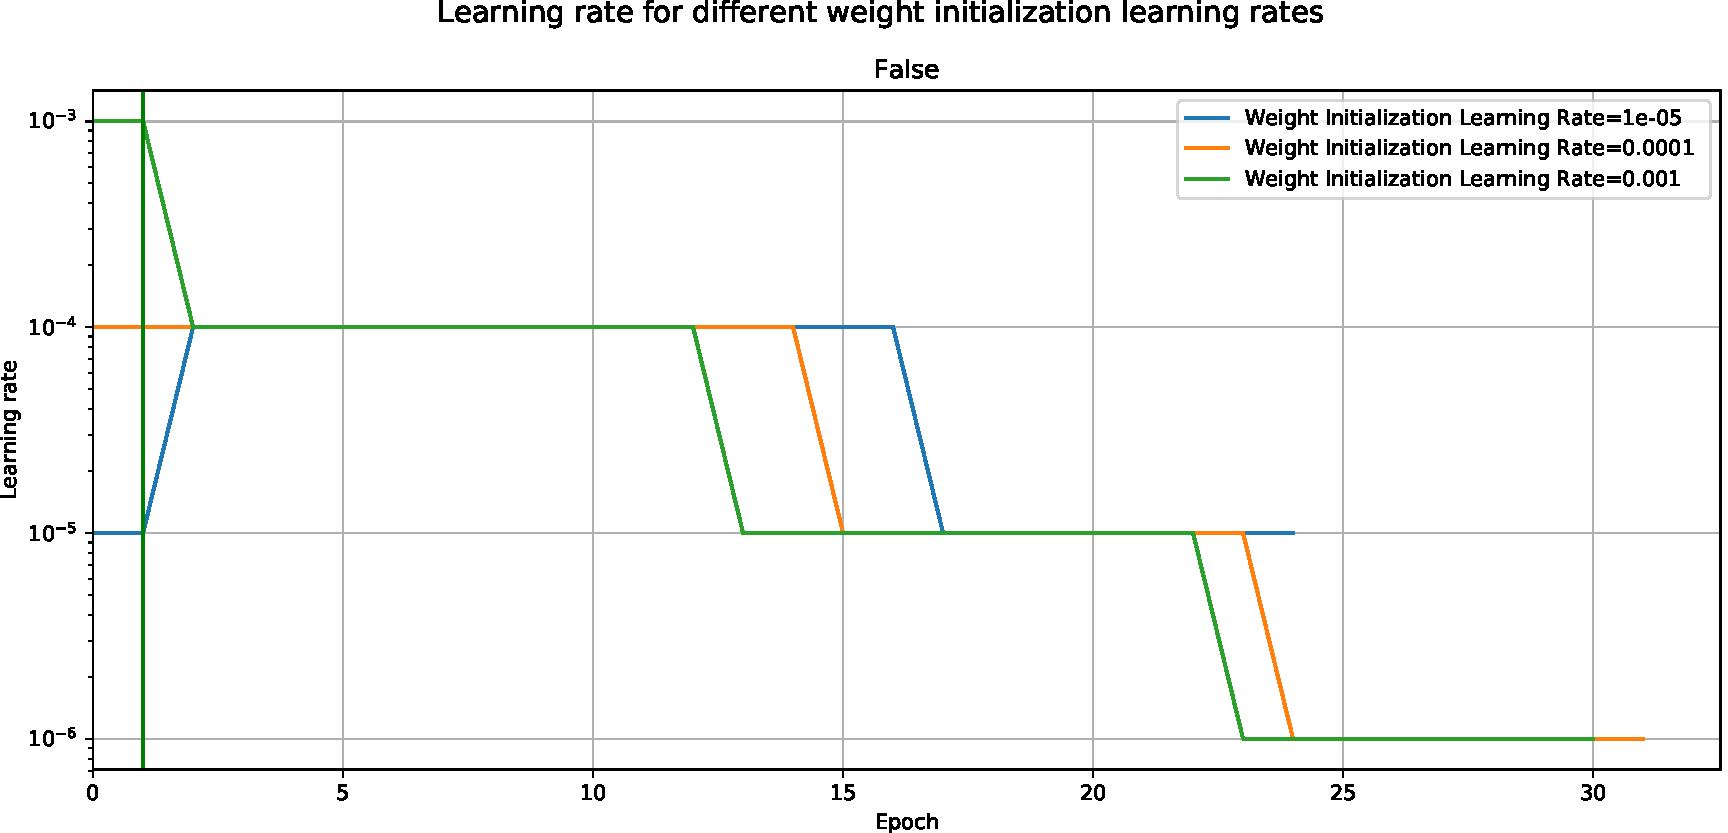
\includegraphics[width=\textwidth]{figs/densenet201_wilr_lr_over_epochs.pdf}
        \caption{Influence of weight initialization learning rate on the evolution of learning rate over epochs}
        \label{fig:wilr_lr_over_epochs}
    \end{figure}
    
    The most impactful learning rate is the start fine tuning learning rate which is used to fine tune the whole model after the weights of the classifier had been initialized. Hypothetically, choosing too small learning rate values will result in a long training process that could get stuck in a local minimum, whereas a value too large may result in learning a sub-optimal set of weights too fast or an unstable training process. We verify this hypothesis by comparing various fine tuning learning rates, which are compared in Figure \ref{fig:ftlr_comp}. \par
    \begin{figure}[ht]
        \centering
        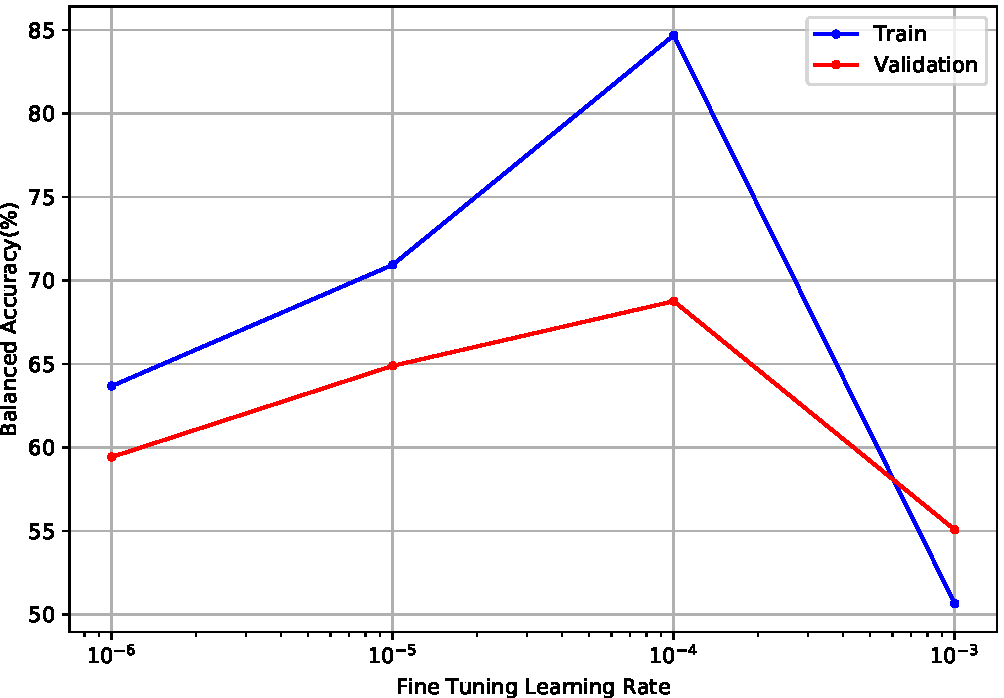
\includegraphics[width=0.6\textwidth]{figs/densenet201_ftlr_comp.pdf}
        \caption{Influence of fine tuning learning rate on train and validation balanced multi-class accuracy}
        \label{fig:ftlr_comp}
    \end{figure}
    
    Figure \ref{fig:ftlr_bma_over_epochs} shows that a low learning rate like $1^{-6}$ make the improvements  linear, while higher learning rates like $1^{-4}$ tend to show a more exponential curve because they will decay the loss faster. However, when the learning rates are too big they can get stuck at worse values of loss which is the case of $1^{-3}$. This is because there is too much "energy" in the optimization and the parameters are bouncing around chaotically, unable to settle in a nice spot in the optimization landscape. \par
    The learning rate of $1^(-4)$ seems to be the optimal choice because it allows the model to have a higher chance of finding a better region of search space in the initial epochs, which consequently influences the rest of the training process because the rest of the epochs will be spent on minimizing the loss within that specific region, that is finding the local minimum. In contrast, learning rates like $1^{-5}$ and $1^{-6}$ have a lower chance of finding a good local minimum at the beginning of the training process and therefore take more epochs to converge, and higher learning rates like $1^{-3}$ are too big such that the network never finds a good region of search space at the beginning of the training process, which influences the rest of the training because the latter lower learning rates will try to optimize the loss within a bad search space. \par
    
    \begin{figure}[ht]
        \centering
        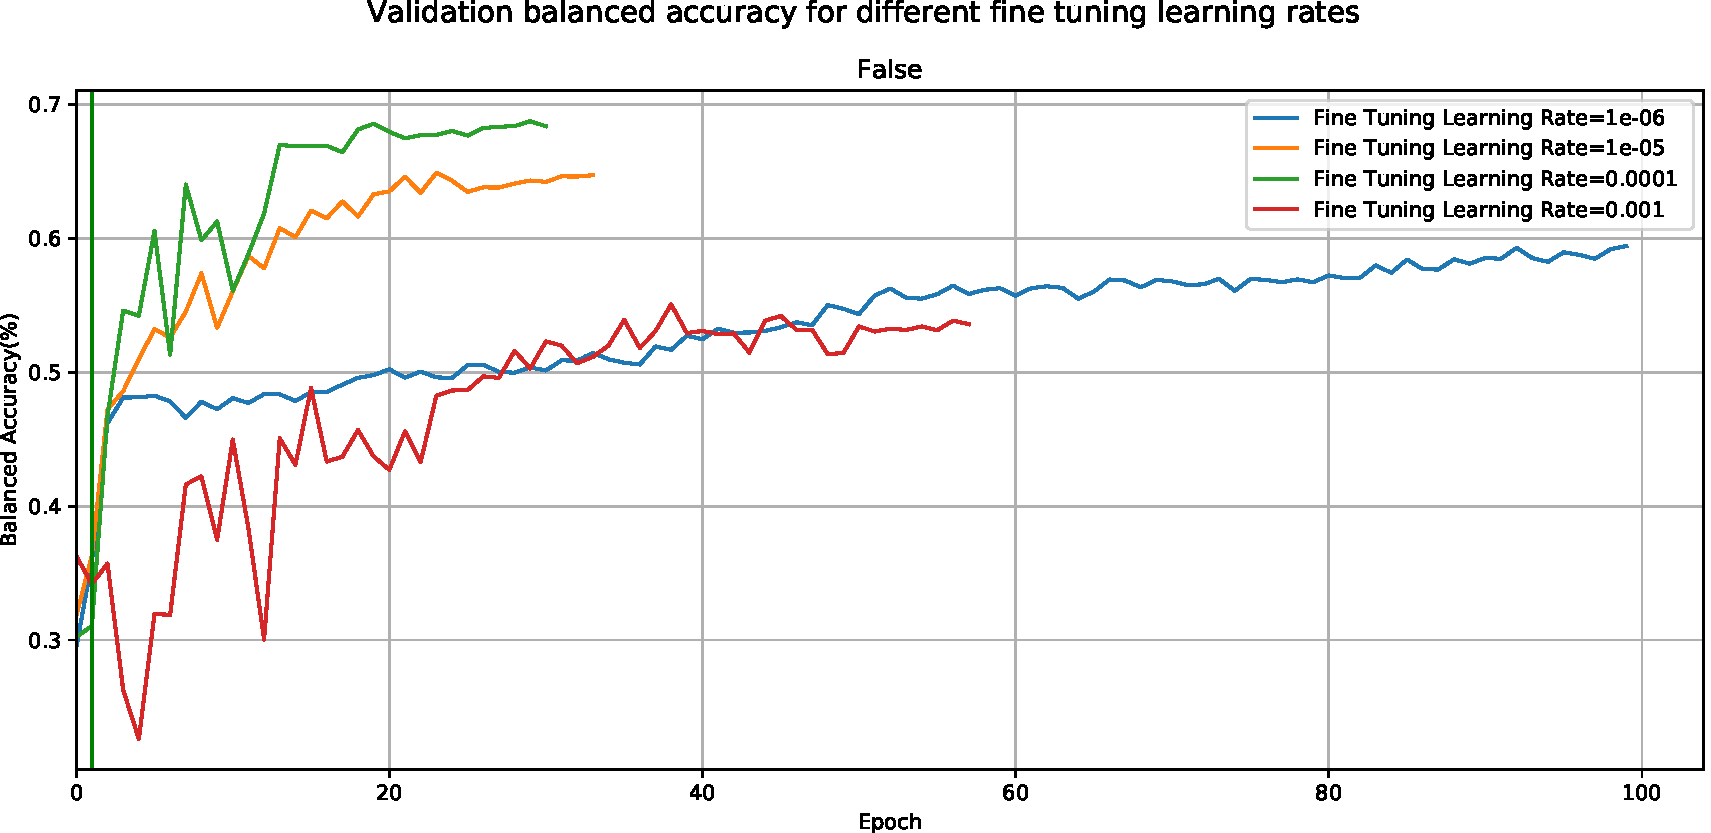
\includegraphics[width=\textwidth]{figs/densenet201_ftlr_bma_over_epochs.pdf}
        \caption{Influence of fine tuning learning rate on train and validation balanced multi-class accuracy over epochs}
        \label{fig:ftlr_bma_over_epochs}
    \end{figure}
    \begin{figure}[ht]
        \centering
        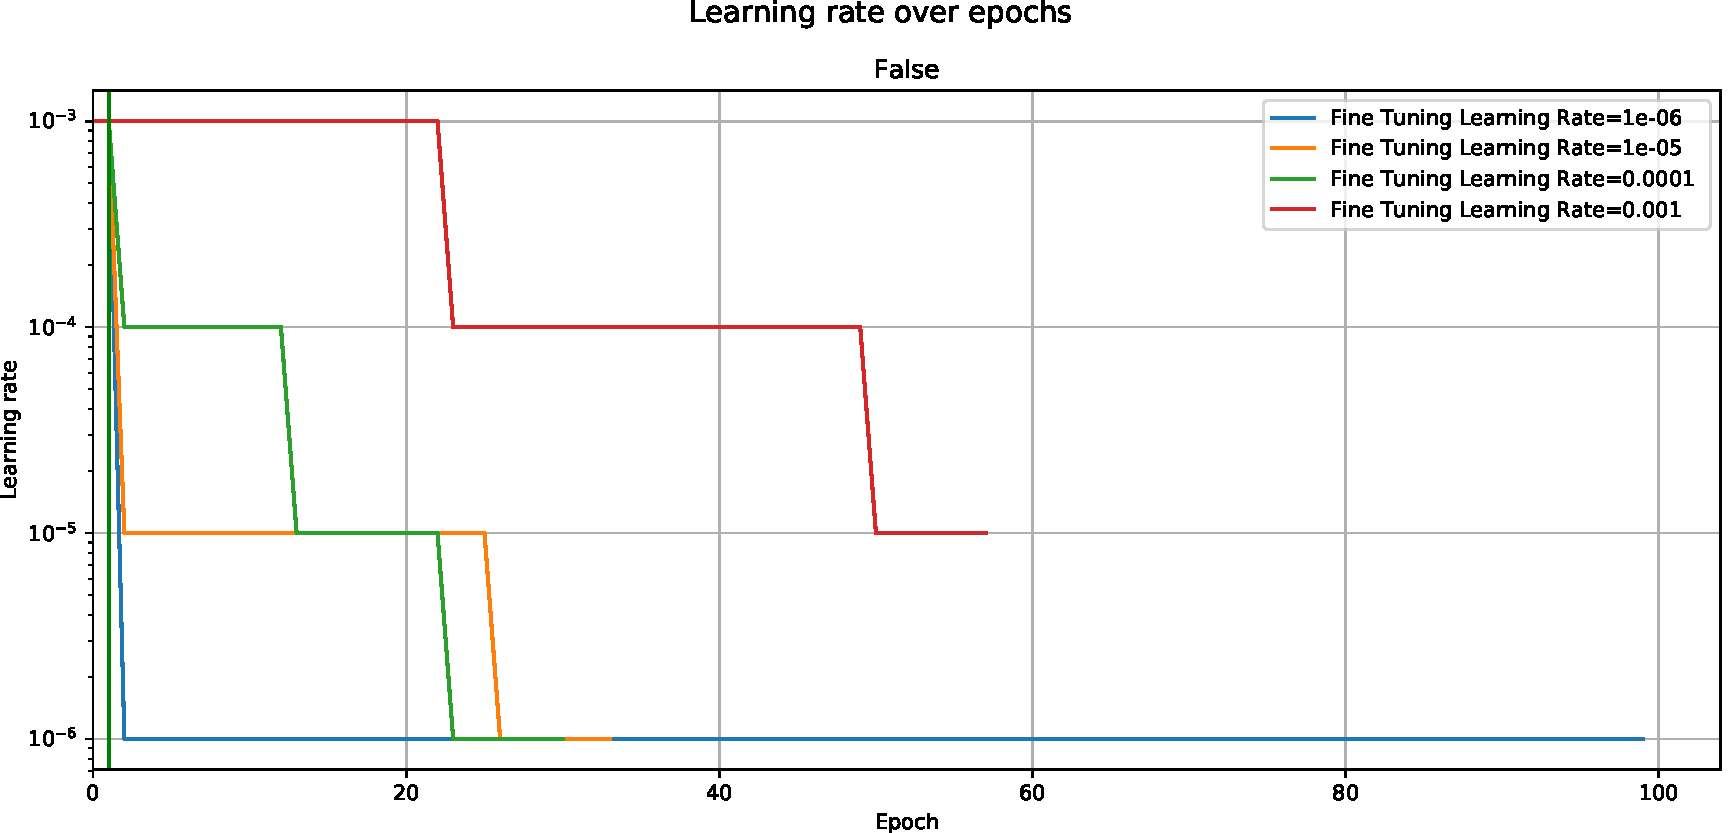
\includegraphics[width=\textwidth]{figs/densenet201_ftlr_lr_over_epochs.pdf}
        \caption{Influence of fine tuning learning rate on the evolution of learning rate over epochs}
        \label{fig:ftlr_lr_over_epochs}
    \end{figure}
    
    From in \ref{fig:ftlr_comp}), one can see that even for the chosen hyperparameters the model still suffers from overfitting, as seen by the huge discrepancy between training and validation balanced multi-class accuracy. In light of the problem, l2 regularization was used, which adds a cost to the loss function of the network for large weights (or parameter values), and presumably result in a overall simpler model that will be forced to learn only the relevant patterns in the train data. However, results (see \ref{fig:densenet201_lambda_comp}) show worse overall performance. Other techniques such as dropout were also experimented with (see \ref{fig:densenet201_dropout_comp}), but again no significant improvements were to be shown. \par 
    \begin{figure}[ht]
        \centering
        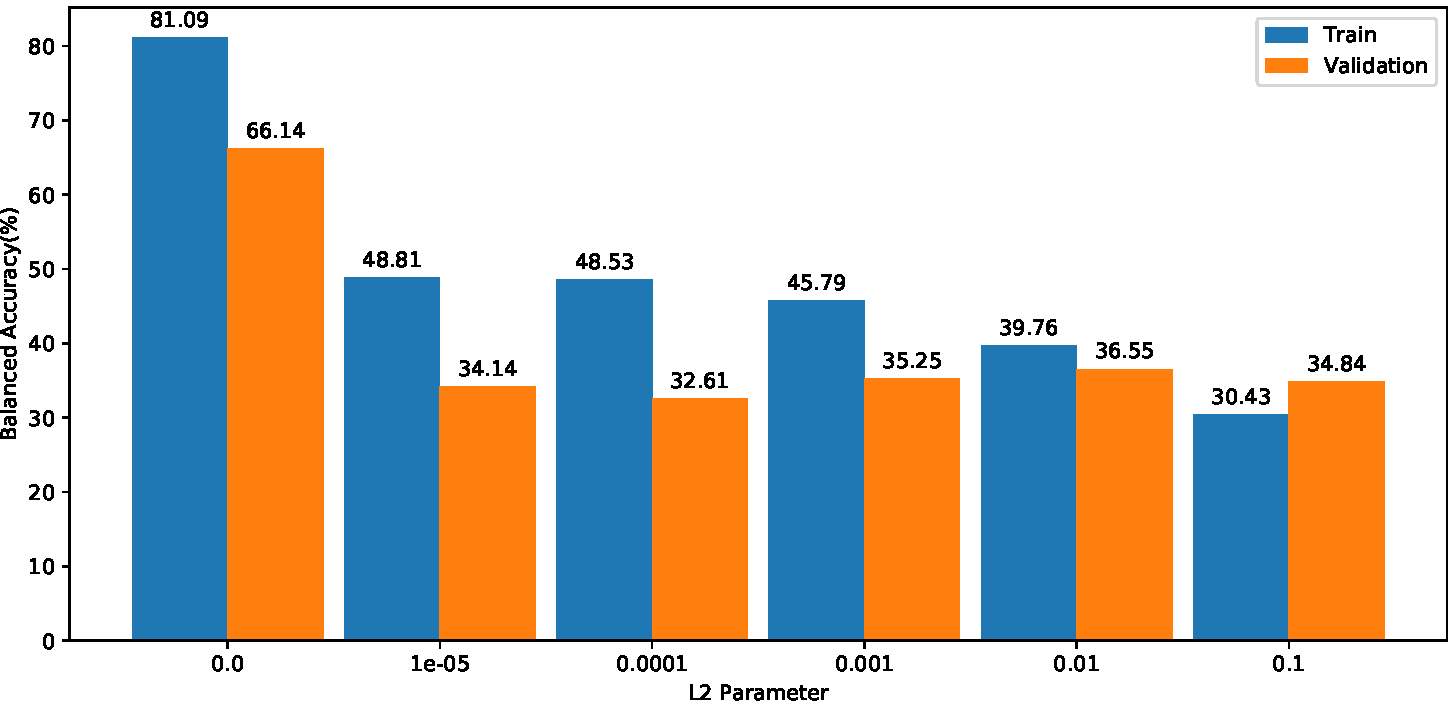
\includegraphics[width=\textwidth]{figs/densenet201_lambda_comp.pdf}
        \caption{Influence of l2 regularization parameter on train and validation balanced multi-class accuracy}
        \label{fig:densenet201_lambda_comp}
    \end{figure}
    
    \begin{figure}[ht]
        \centering
        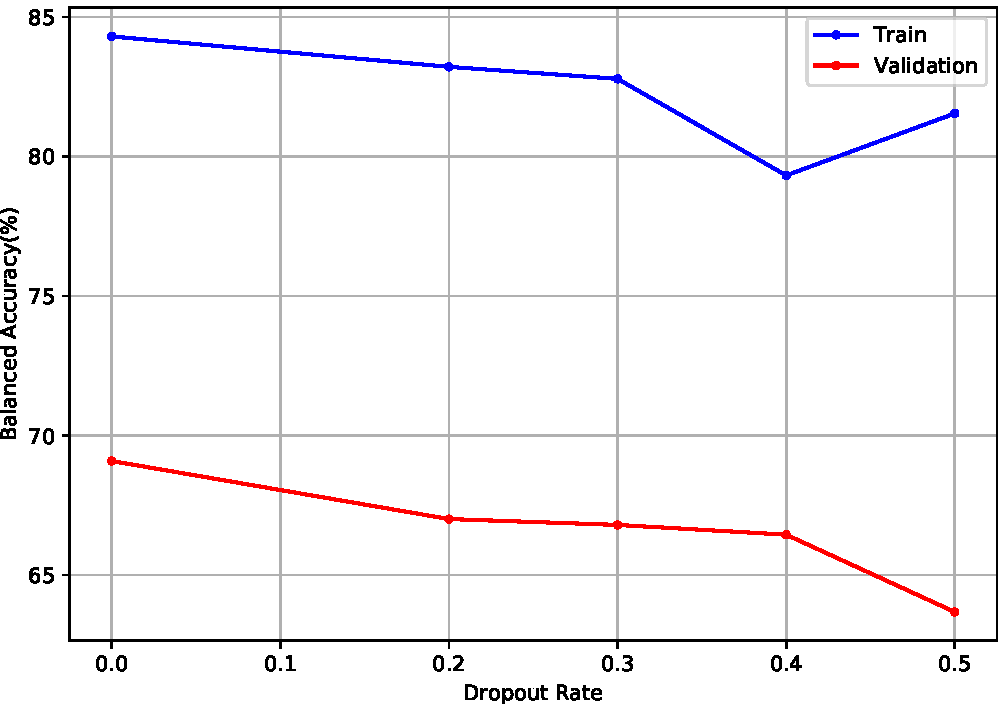
\includegraphics[width=0.6\textwidth]{figs/densenet201_dropout_comp.pdf}
        \caption{Influence of dropout rate on train and validation balanced multi-class accuracy}
        \label{fig:densenet201_dropout_comp}
    \end{figure}
    
    DenseNet201 has a considerably large number of trainable parameters when compared with other models such as  (see \ref{tables:pretrainedmodels}), which in theory means that it is easier for the model to memorize samples, and therefore overfit. As such, by lowering the capacity of the network, one will force it to learn the patterns that matter or that minimize the loss. To put this into test, results for variations with a smaller number of parameters of the DenseNet, specifically, DenseNet121 and DenseNet169, were compared with DenseNet201 in Figure \ref{fig:densenet_variations_5000_comp}. Results show that indeed lowering the network's capacity improves performance, but not by a significant margin.
    \begin{figure}[ht]
        \centering
        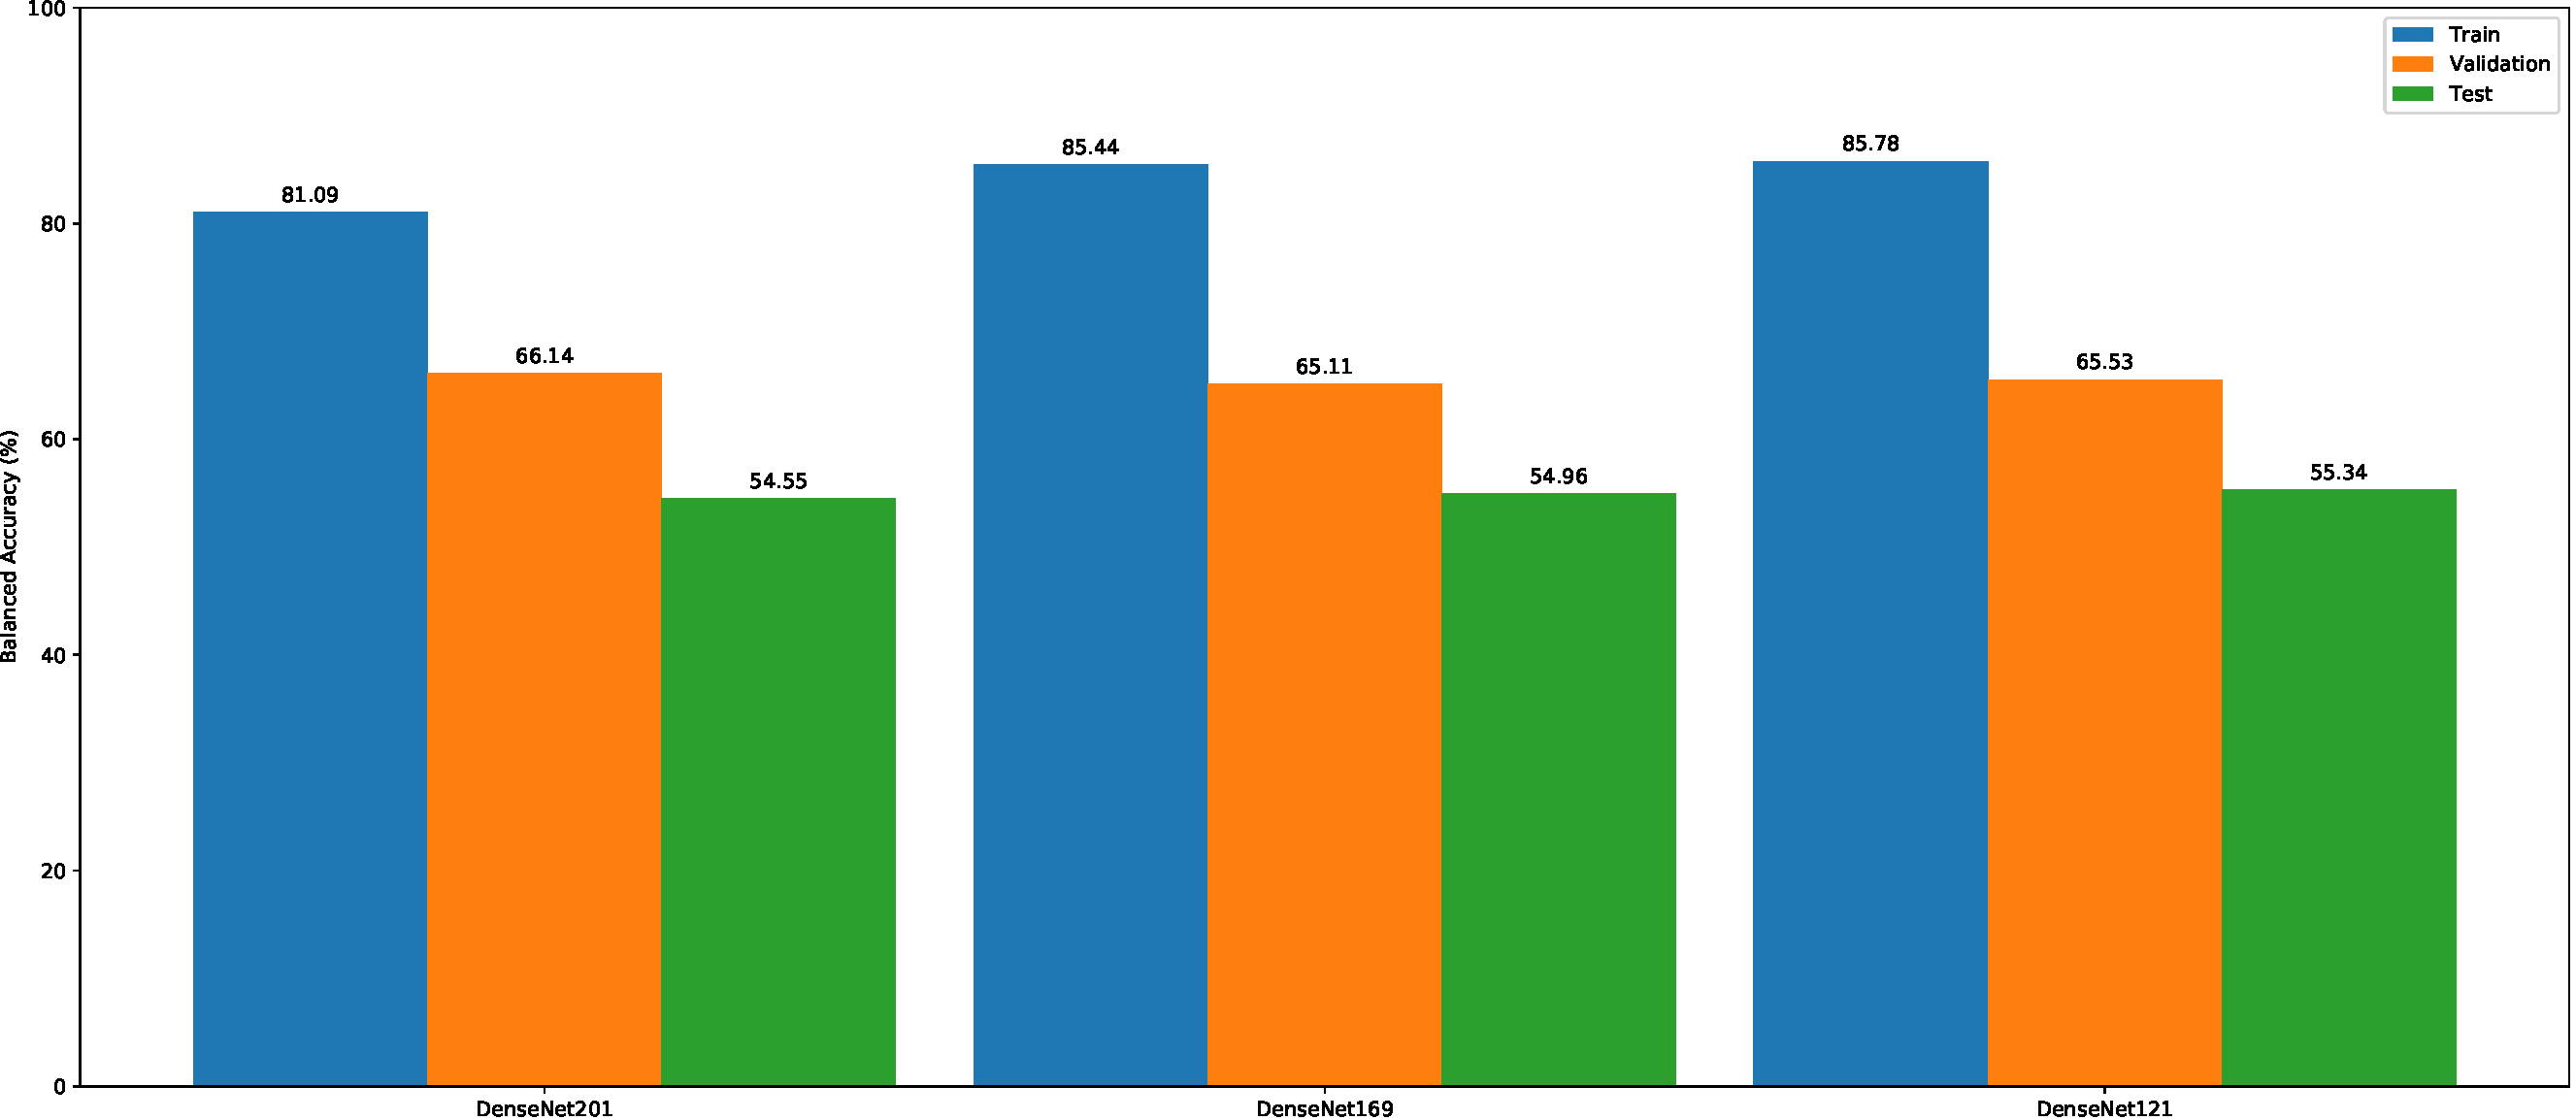
\includegraphics[width=\textwidth]{figs/densenet_variations_5000_comp.pdf}
        \caption{Comparison of different variations of DenseNet on train, validation and test balanced multi-class accuracy for a dataset with 5000 unbalanced samples}
        \label{fig:densenet_variations_5000_comp}
    \end{figure}
    
    With the parameters now set the model is now able to get accuracy of $75.4\%$ and a balanced multi-class accuracy of $59.1\%$. The values of the balanced multi-class accuracy are low relative to the accuracy because some classes have poor performance in comparison with other classes (this effect is shown in the confusion matrix of Figure \ref{?}), which the accuracy metric does not take into account. One can. Overall, the attained performance values so far are relatively low. \par
    \begin{figure}[ht]
        \centering
        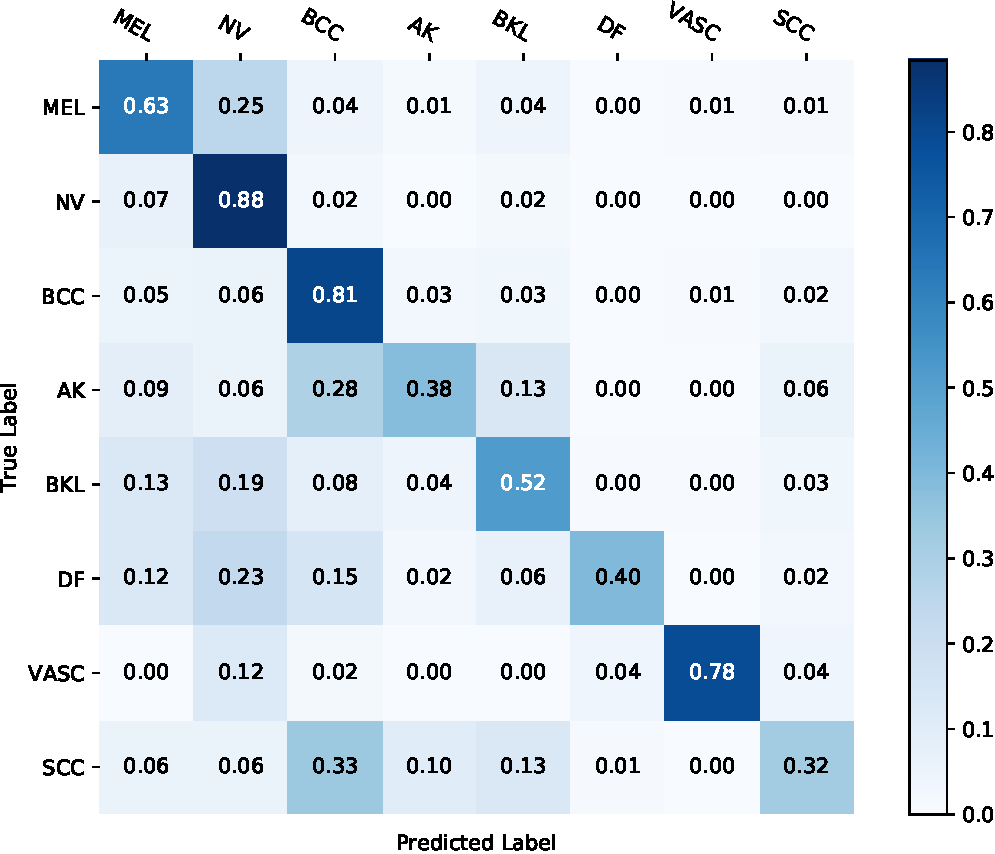
\includegraphics[width=0.6\textwidth]{figs/densenet201_5000_tuned_conf_matrix.pdf}
        \caption{Confusion matrix of the hyperparameter tuned DenseNet201}
        \label{fig:hyperparameter_tuned_conf_matrix}
    \end{figure}
    
\section{Data study} \label{section:balance}
    The validation curve of the hyperparameter tuned model in figure \ref{?} shows a considerable amount of overfitting, as the $BMA_{validation}$ does not approximate $BMA{train}$. Presumably, these results stem from an inappropriate number of training samples relative to the number of free parameters in the network. The dataset used so far has been an undersampled version of the ISIC 2019 challenge dataset, specifically with 4000 training samples and 1000 validation samples that keep the same class distribution as the original ISIC 2019 challenge dataset. This means that underrepresented classes like dermatofibroma or vascular lesion (see Figure  \ref{fig:distribution}) have too few samples to learn strong generalizable features. Indeed, an increase in dataset size enables the DenseNet201 model to overfit less and attain better $BMA_{validation}$ values (see \ref{fig:samples_comp}), which corroborates the importance of data quantity for training deep neural networks.   \par
    
    \begin{figure}[ht]
        \centering
        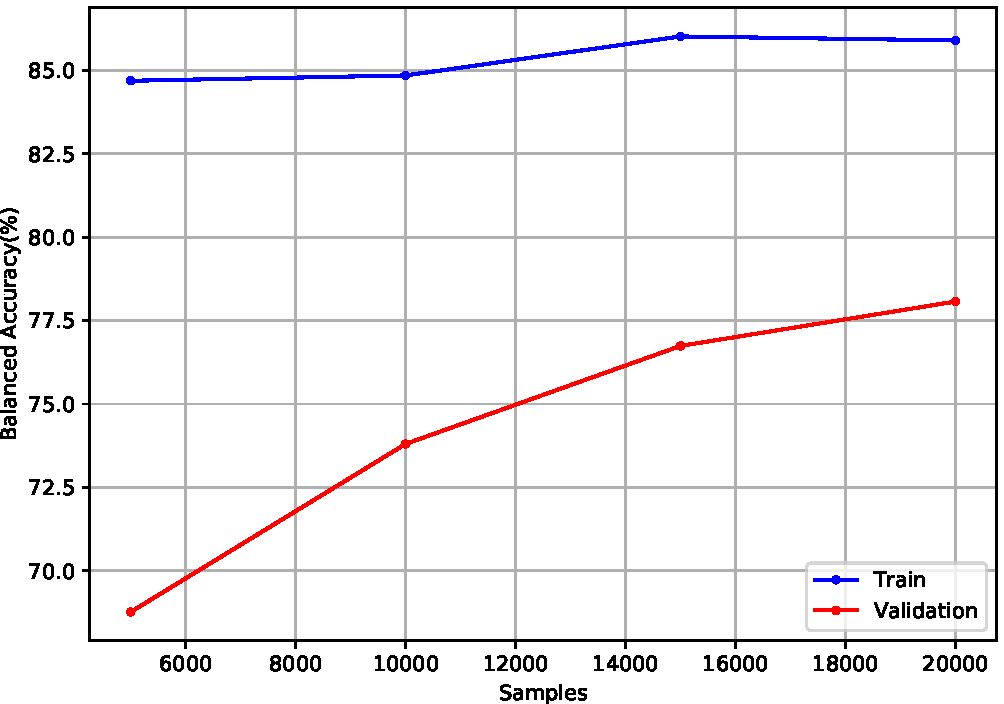
\includegraphics[width=0.6\textwidth]{figs/densenet201_samples_comp.pdf}
        \caption{Influence of the number of samples on the best values of balanced multi-class accuracy of train and validation sets}
        \label{fig:samples_comp}
    \end{figure}
    
    The results from the plot graph in Figure \ref{fig:densenet_variations_5000_comp} showed that one could use a  smaller pre-trained model from DenseNet, while maintaining similar performance, which would overall be benefitial to reduce overfitting. However, with a bigger dataset one could argue that the gap between models with high and low number of trainable parameters would increase. but that is still not the case (see Figure \ref{fig:densenet_variations_20264_comp}). Even though DenseNet201 got the best performance in comparison with it's smaller versions, this improvement is unsubstantial as the difference between the DenseNet121 and DenseNet201 on test data is about ?\%. Considering the results, that difference becomes even more irrelevant when taken into consideration that the gap between train and validation on DenseNet121 is substancially smaller than the one of DenseNet201. As such, a smaller model proves to be a better choice as it reduces overfitting while keeping similar performance to bigger models. \par
    
    \begin{figure}[ht]
        \centering
        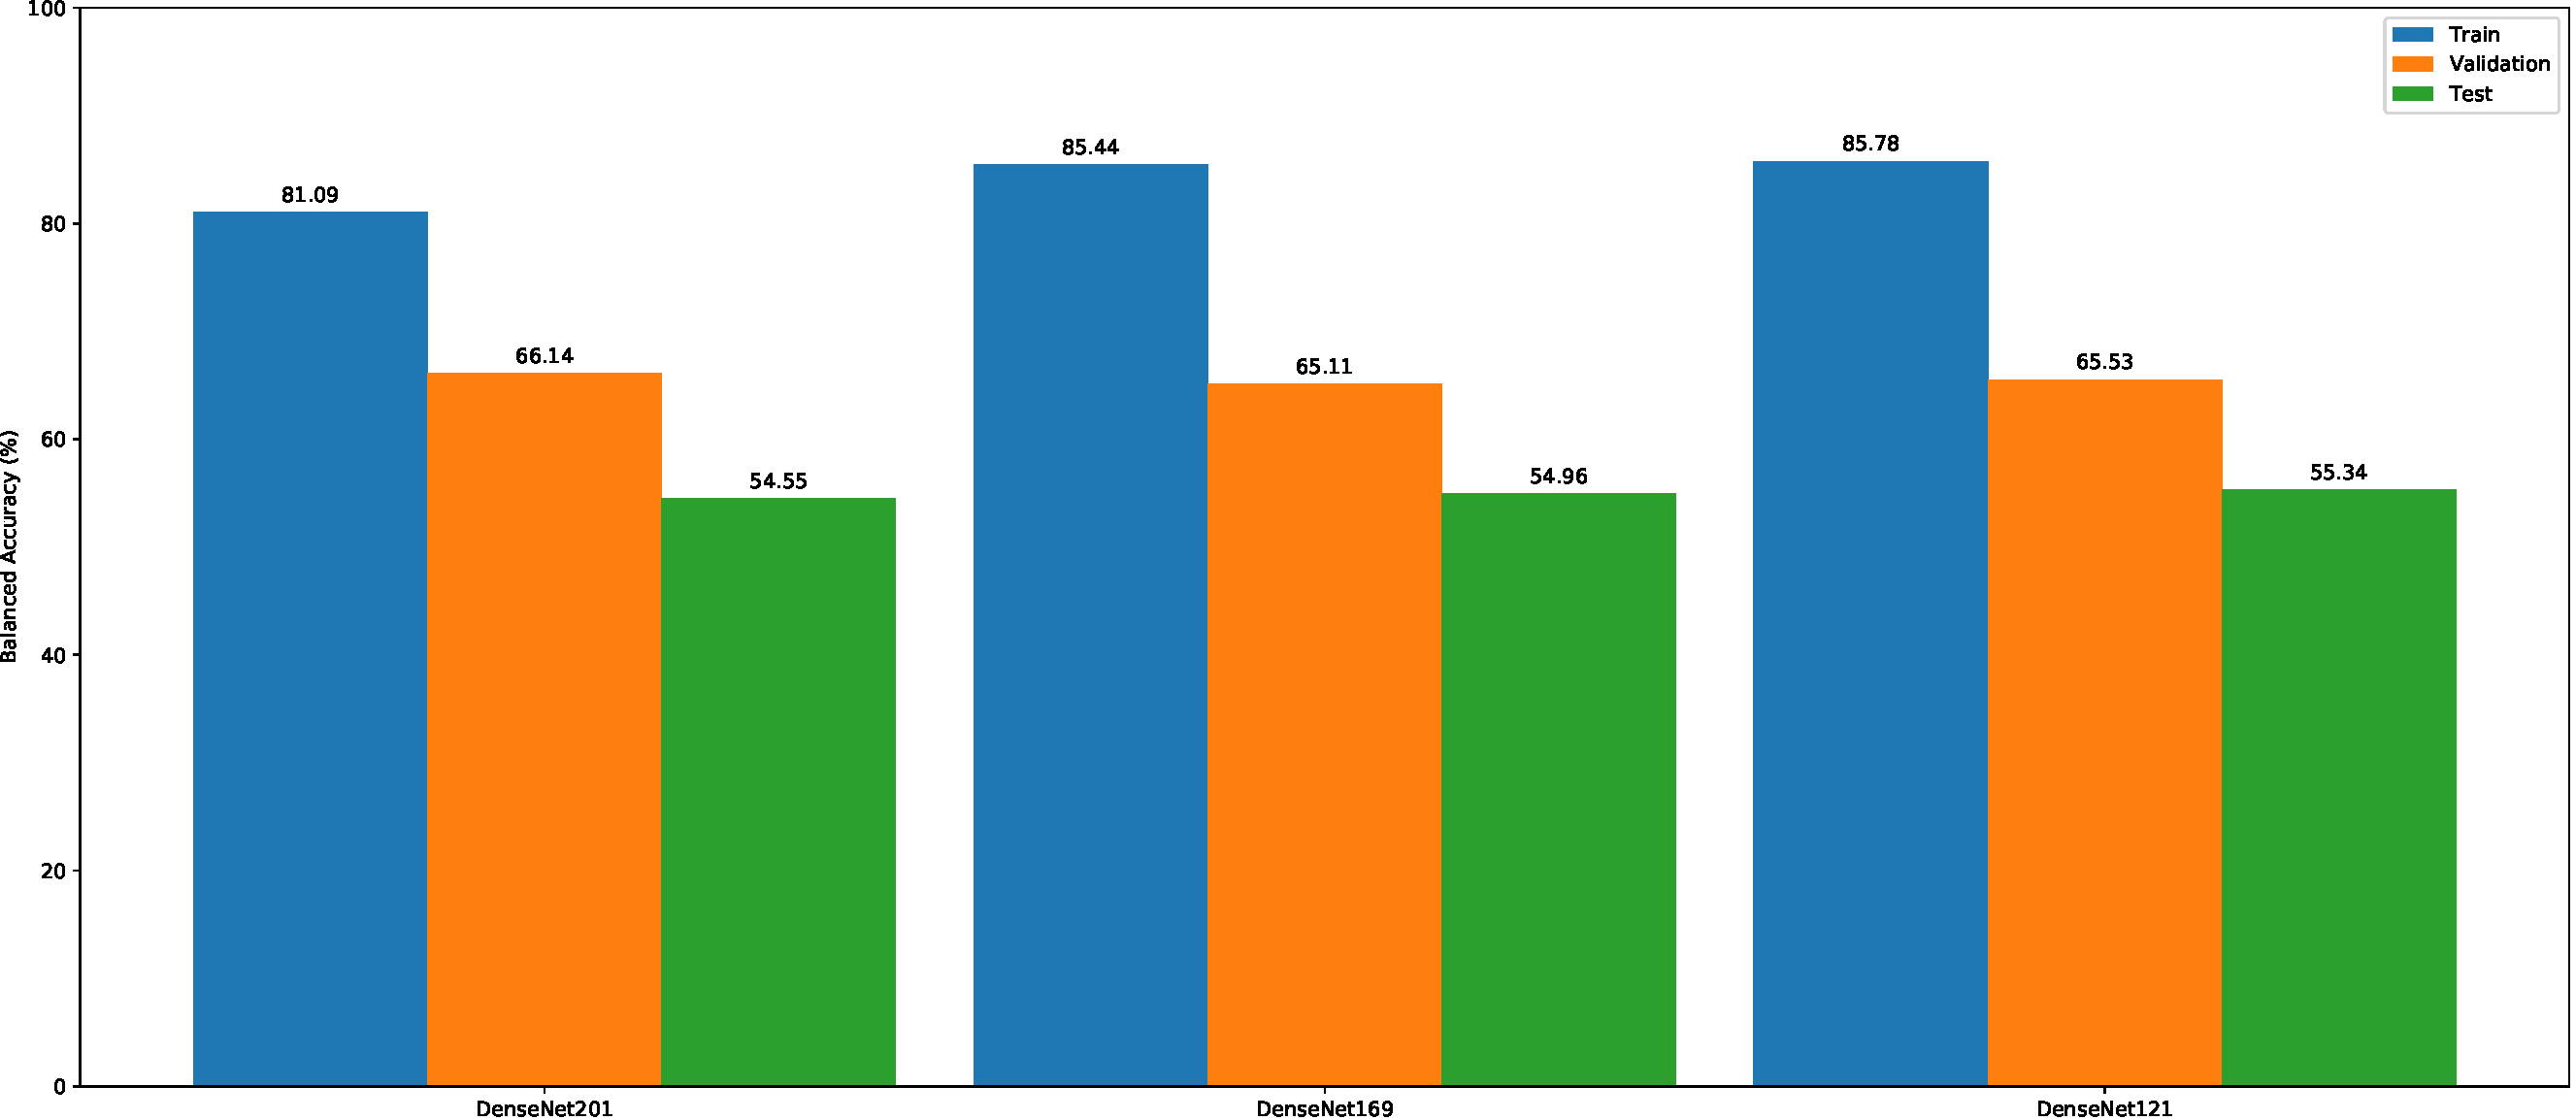
\includegraphics[width=\textwidth]{figs/densenet_variations_20264_comp.pdf}
        \caption{Comparison of different variations of DenseNet on train, validation and test balanced multi-class accuracy for a dataset with 20264 unbalanced samples}
        \label{fig:densenet_variations_20264_comp}
    \end{figure}
    
    From Figure \ref{fig:samples_bma_over_epochs}, one can see that training with more samples takes longer, which is mainly due to the learning rate scheduler. In models with more samples, validation loss keeps improving for longer for higher learning rates, which makes the scheduler decrease the learning rate later compared to models trained with less samples (see Figure \ref{fig:samples_lr_over_epochs}). Consequently, as most models converge to local minimums with low learning rates, models trained with more samples take longer to converge because they take longer to reach low learning rates. \par
    
    \begin{figure}[ht]
        \centering
        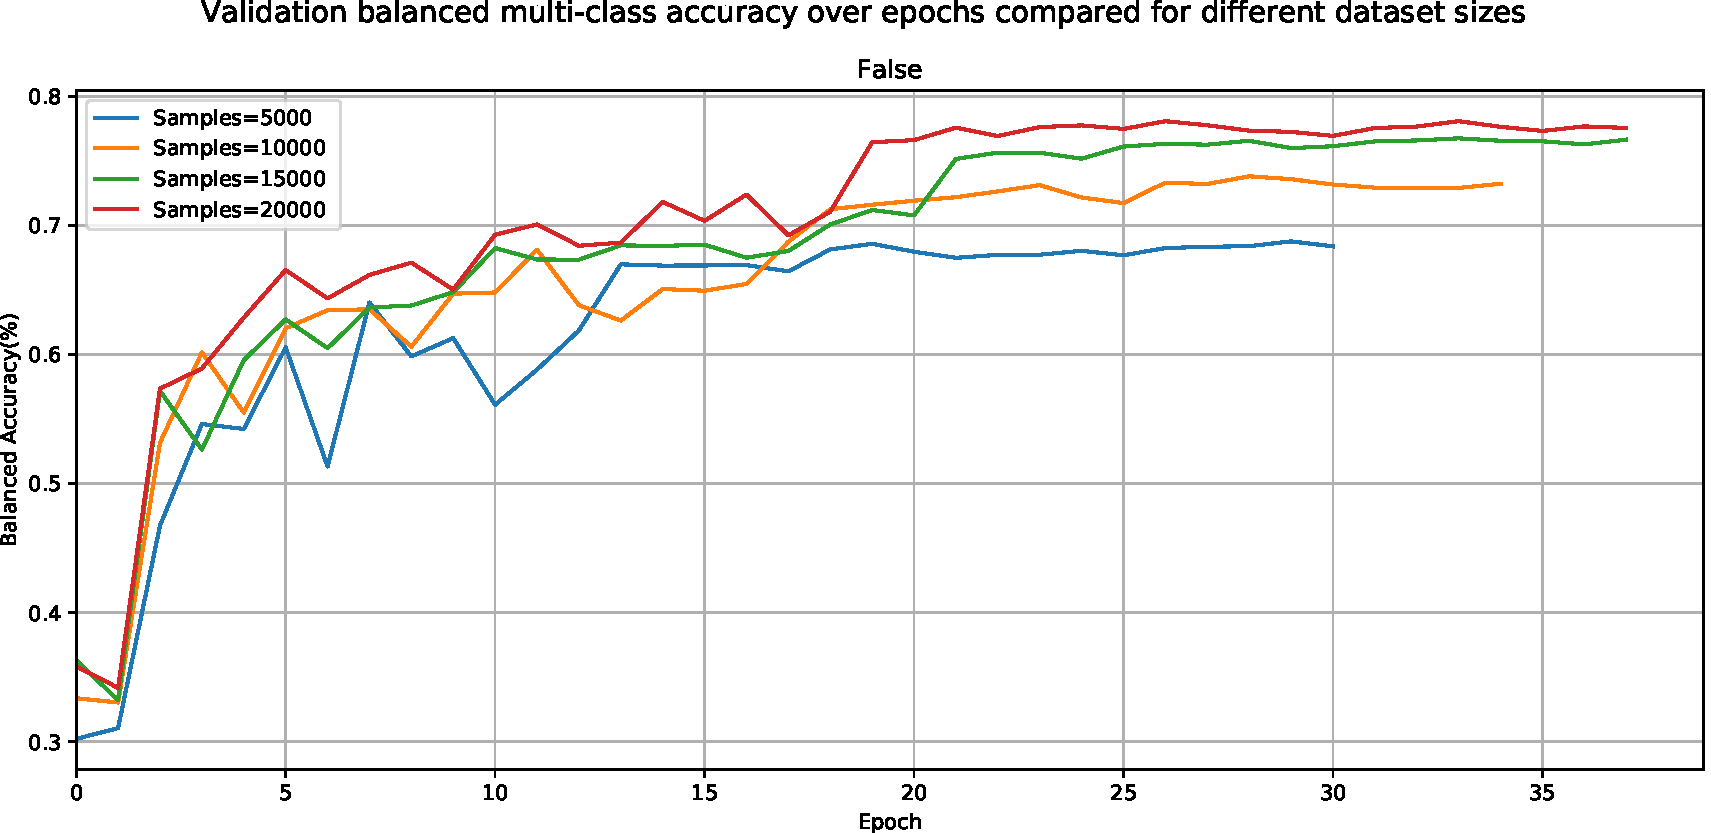
\includegraphics[width=\textwidth]{figs/densenet201_samples_bma_over_epochs.pdf}
        \caption{Influence of the number of samples on validation balanced multi-class accuracy over epochs}
        \label{fig:samples_bma_over_epochs}
    \end{figure}
    \begin{figure}[ht]
        \centering
        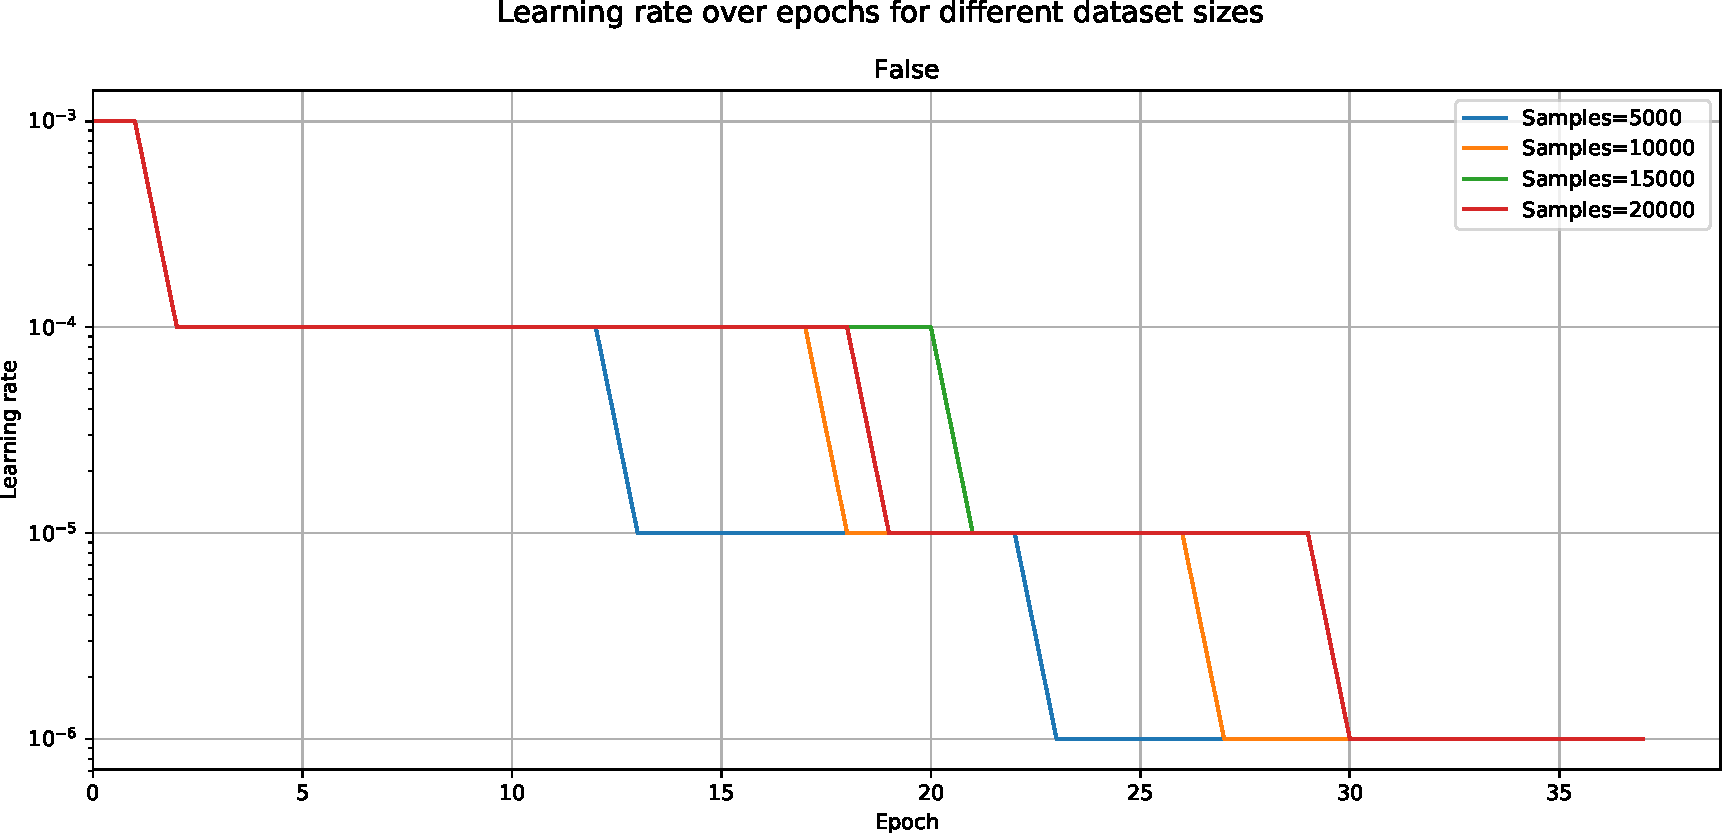
\includegraphics[width=\textwidth]{figs/densenet201_samples_lr_over_epochs.pdf}
        \caption{Influence of the number of samples on the learning rate over epochs}
        \label{fig:samples_lr_over_epochs}
    \end{figure}
    
    Considering the results from \ref{fig:samples_comp}, there is a considerable improvement on the overall performance by increasing the dataset. Virtually one could assume that increasing the dataset size through other techniques such as data augmentation could improve the overall performance of the network, specially in underrepresented classes. Different strategies of data augmentation can be used, one of them being offline data augmentation, meaning that a bigger dataset is generated before the training process from an original dataset through augmentation techniques. However, there are different methods for augmenting images such as rotations or distortions and they can be combined together to produce images which are substancially different from their originals. As such, depending on the number of augmentations to be considered there could be a huge amount of different combinations between them specially considering that some of them have different variations and parameters which can quite change the augmentation (the magnitude of a distortion or the angle of a rotation). Therefore, it is important to determine what combinations of data augmentation techniques significantly improve the overall performance for the problem of skin lesion classification. \par
    
    Figure \ref{fig:data_aug_group_bal_acc_comp} shows a comparison between different augmentation groups applied to the hyperparameter tuned DenseNet201 obtained from \autoref{section:hyperparameters} with 20264 class balanced samples (2533 per class), meaning that underrepresented classes are oversampled through the augmentation techniques from each of the groups, and overrepresented classes are undersampled by choosing samples randomly from that class without repetition. In turn, this means that only ?????x samples are oversampled and the rest of the images are original ones. The presented groups are:
    \begin{itemize}
        \item Group 0: No augmentation techniques are applied. Oversampling is done by randomly copy and pasting samples from a specific class with repetition. This is the baseline which other groups should be compared against.
        \item Group 1: Composed of rotations of 90 degrees, flips from top to bottom or vice versa, flips from left to right or vice versa, not centered crops that keep 85\% of the original size and shears with a variation anywhere from 20 degrees towards the left side of the image to 20 degrees towards the right side of the image. 
        \item Group 2: Composed of the augmentation techniques of group 1 plus some adjustments on pixel intensities, specifically, brightness changes from 50\% to 150\% (100\% being the original image and 0\% being a black image), contrast changes from 50\% to 150\% (100\% being the original image and 0\% being a solid grey image), and coloration changes from 50\% to 150\% (100\% being the original and 0\% being a black and white image).
        \item Group 3: Composed of the augmentation techniques of group 1 plus perspective transformations. These transformations include tilts on either the left or right side, tilts forward and backward and skews from a random corner of an image.
        \item Group 4: Composed of the augmentation techniques of group 1 plus noise induction augmentation techniques. Elastic distortions are applied with a grid size of 8, meaning that the image is divided into 8x8 cubes and each region is distorted independently. Random erasing is also applied, which takes a random area equivalent to 25\% of the original image and replaces it by random pixels, meaning that each pixel has a random intensity producing noise in that area.
    \end{itemize}
    In group 1, 2, 3 and 4 there is a probability of 0.5 of applying a specific augmentation technique in the group augmentation pipeline, which means that the same sample augmented multiple times will likely produce different augmented samples. This is a desirable property as producing the same synthetic sample over and over again would produce a lot of repetition in highly undersampled classes, and eventually lead to problems like overfitting as in each epoch the network would minimize loss for the same repeated sample, rather than learning from variations of that sample. \par
    
    Considering the results from Figure \ref{fig:data_aug_group_bal_acc_comp}, overall data augmentation does improve the performance in comparison with group 0, which does not employ any type of augmentation. Moreover, it seems the simpler augmentation approaches like group 1 and 2 perform the best, while more complex augmentations groups such as group 3 and 4 perform worst.   \par
    
    This results indicate that more conventional augmentation techniques alone perform better, which does make sense in the context of skin lesion classidicatino. As described in \autoref{chapter:sota} a common method used by dermathologists to identify skin lesions is the ABCDE method, which relies in features like the shape and color of the lesion to be diagnosed. Therefore, by changing such features we are potentially removing or changing important information about the lesion itself, which consequently will make the network perform worst. For instance, group 4 introduces noise inducing transformations, however, one cannot predict if the random erasing will erase important information from the lesion itself or if the distortion performed will alter the shape of the lesion in such a way that it is no longer characteristic of it's category. Similarly, by changing the colors of the lesion in group 2 we are pottentially changing important information about the colour of the lesion which is one of the most important features to consider when diagnosing a lesion \cite{?}.  \par
    
    \begin{figure}[ht]
        \centering
        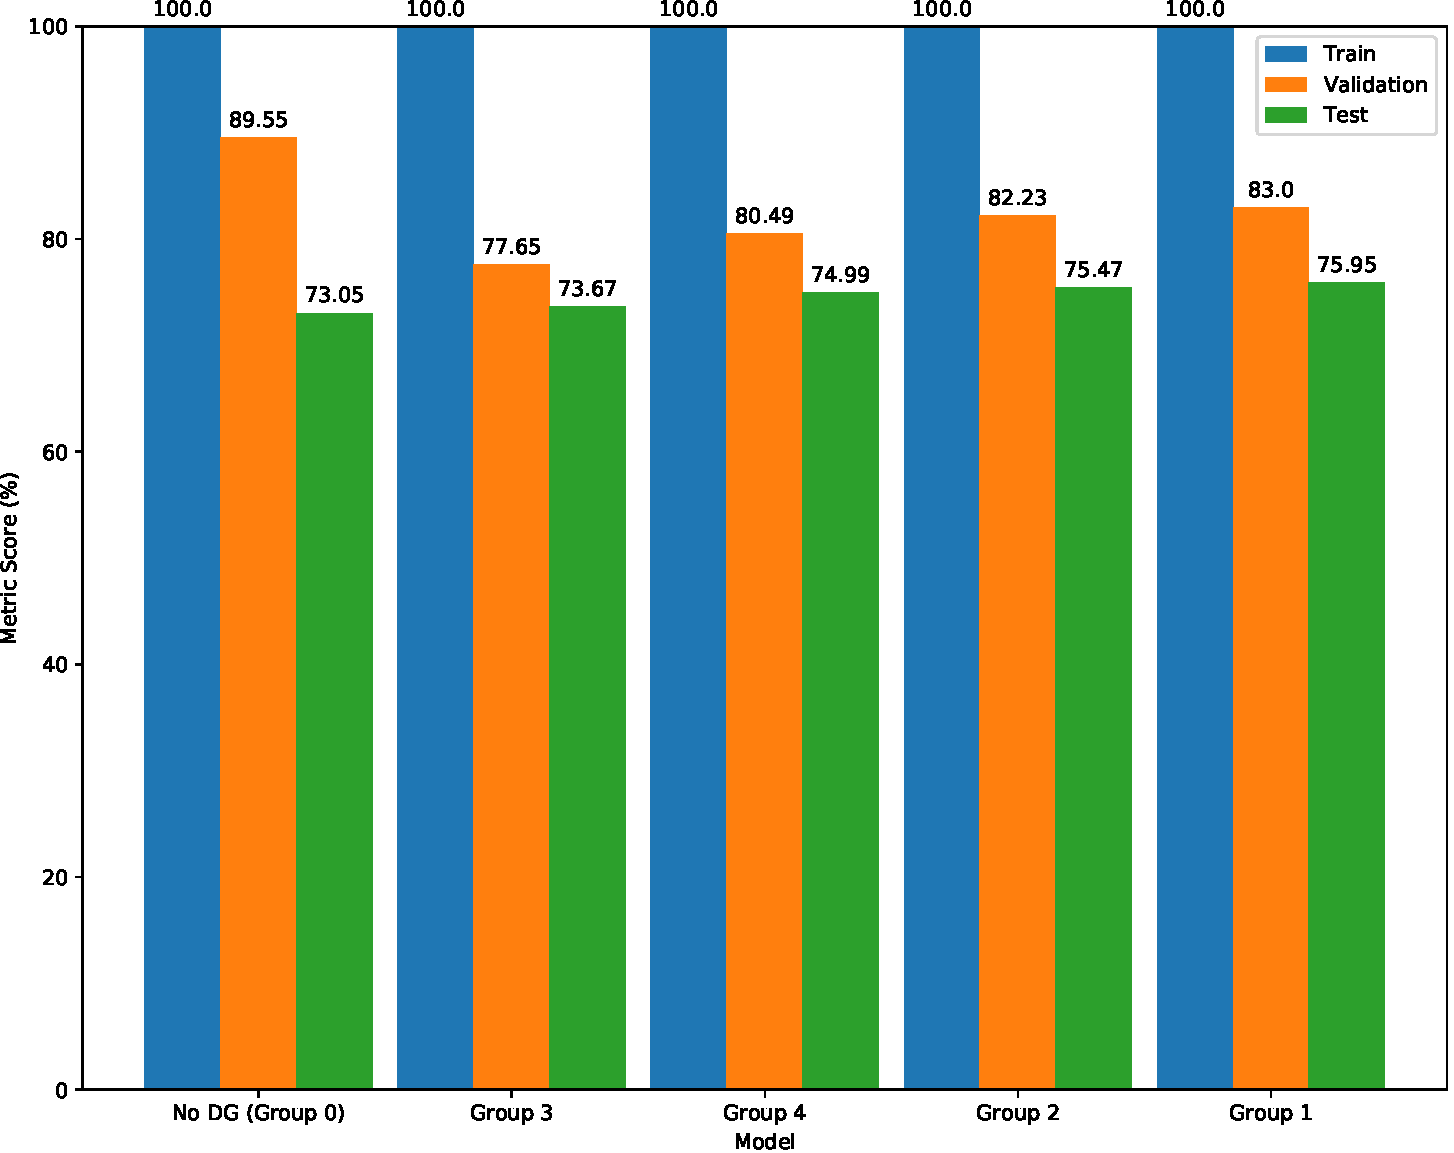
\includegraphics[width=\textwidth]{figs/data_aug_group_bal_acc_comp.pdf}
        \caption{Balanced multi-class accuracy of train, validation and test sets of different offline data augmentation groups with a hyperparameter tuned DenseNet201 trained on 20264 balanced samples}
        \label{fig:data_aug_group_bal_acc_comp}
    \end{figure}
    
    Furthermore, offline data augmentation is not the only method of applying data augmentation, specifically, online data augmentation is from the literature presented in \autoref{chapter:sota} a commonly used technique to reduce overfitting. In fact, as shown in Figure \ref{fig:data_aug_mode_bal_acc_comp}, online data augmentation significantly reduces the gap between train and validation both when employed with offline data augmentation or not, while also significantly increasing test performance. It is important to note that whenever data augmentation is applied in this experiment data augmentation group 1 is being used. \par
    
    \begin{figure}[ht]
        \centering
        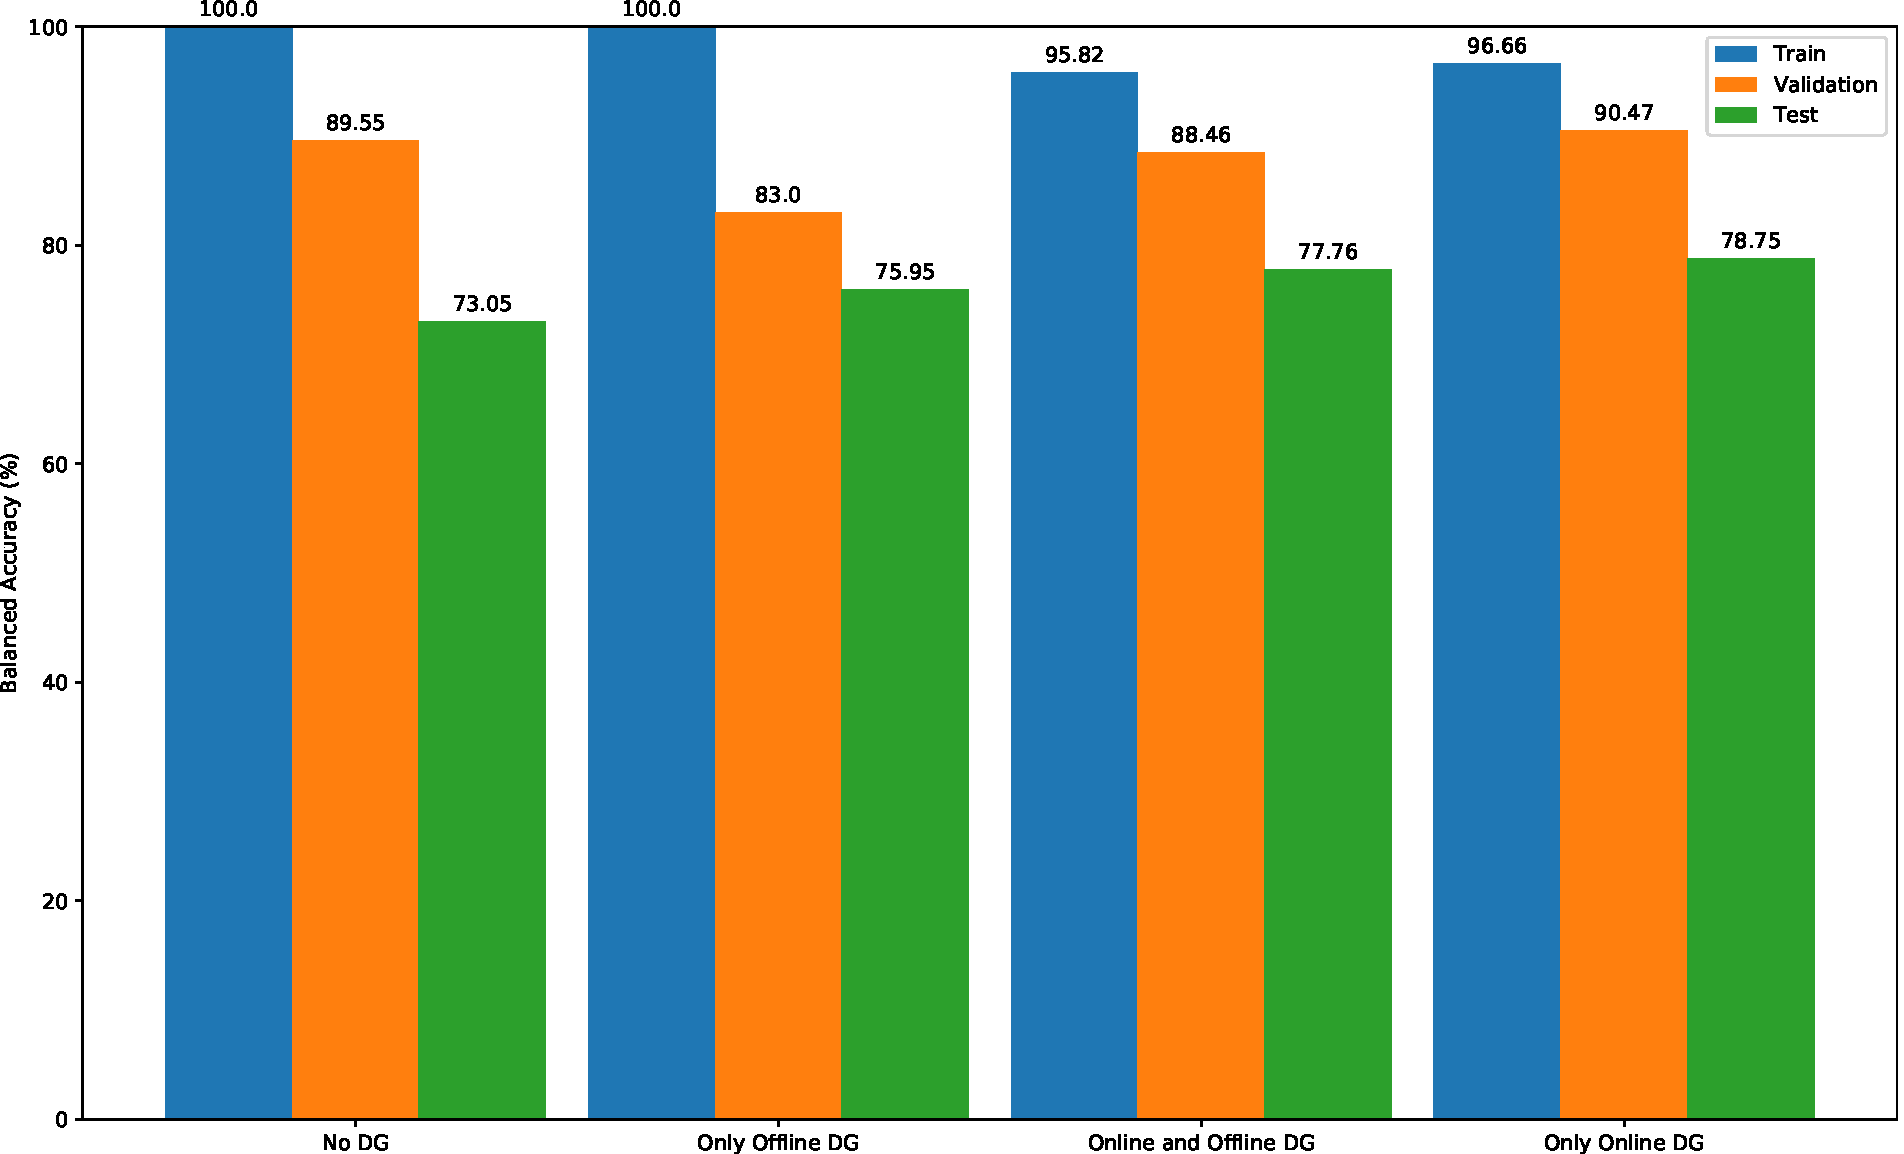
\includegraphics[width=\textwidth]{figs/data_aug_mode_bal_acc_comp.pdf}
        \caption{Balanced multi-class accuracy of train, validation and test sets of different combinations of offline and online data augmentation modes with a hyperparameter tuned DenseNet201 trained on 20264 balanced samples. No data augmentation is equivalent to augmentation group 0, }
        \label{fig:data_aug_mode_bal_acc_comp}
    \end{figure}
    
    So far, results show that classification towards underepresented classes like dermafibroma has overall worse performance than classes like melanocytic nevus (see the confusion matrix from \ref{fig:hyperparameter_tuned_conf_matrix}), which means that there is not enough samples to train a model for it to perform well on these classes. Data augmentation, can alleviate this issue by generating interesting variations of samples that are part of underrepresented classes. For instance, Figure \ref{fig:densenet201_bma_comp} shows an experiment where a balanced model with 2533 samples per class is compared against a unbalanced model of 20264 model by their balanced multi-class accuracy over the train, validation and test datasets. Results show that the balanced model will converge to a better local minimum in respect with all three sets. \par
    
    \begin{figure}[ht]
        \centering
        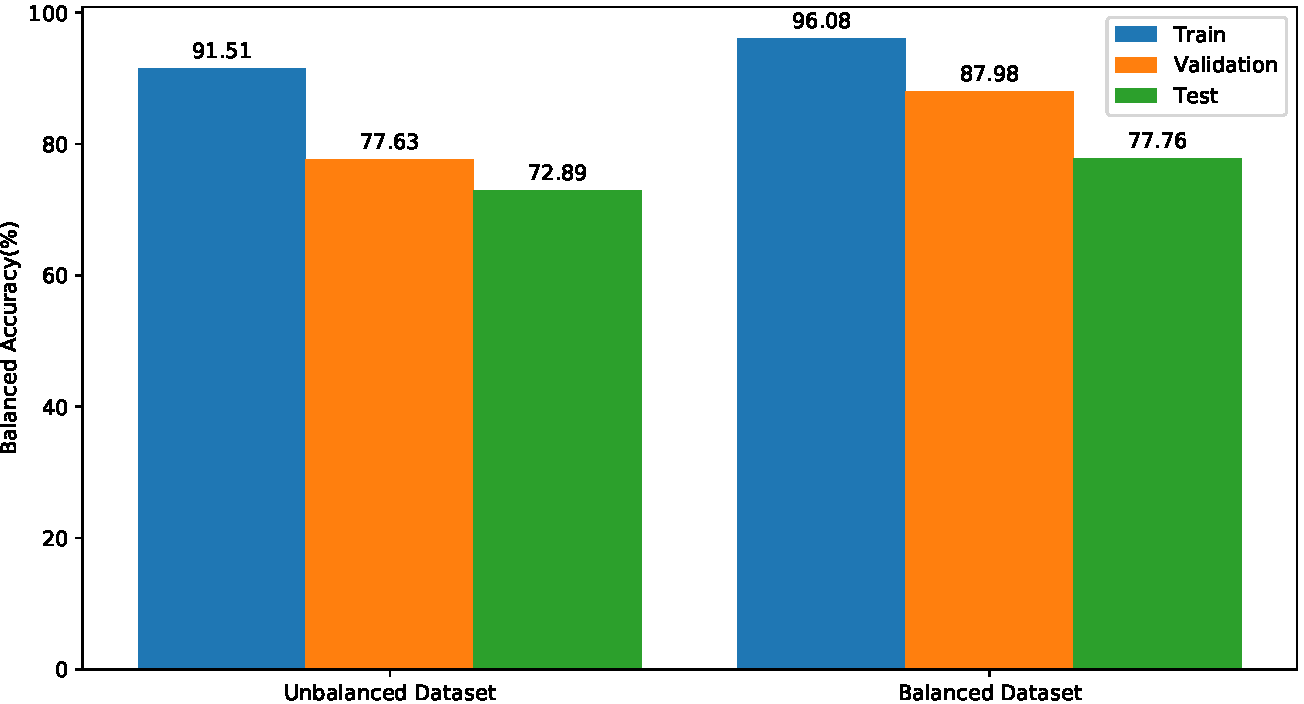
\includegraphics[width=\textwidth]{figs/densenet201_bma_comp.pdf}
        \caption{Comparison of the balanced multi-class accuracy of balanced and unbalanced datasets with 20264 samples for the train, validation and test sets.}
        \label{fig:densenet201_bma_comp}
    \end{figure}
    
    However, by doing the same comparison but with the accuracy metric, results show that the accuracy over the unbalanced dataset are better than those from the balanced dataset (see Figure \ref{fig:densenet201_acc_comp}). It is evident from the results that offline data augmentation is improving performance on underrepresented classes shown by the $BMA$ increase, but by undersampling overrepresented classes, the accuracy takes a hit because these classes get slightly lower performance, which consequently does make a big impact on the accuracy metric as this metric does not average the results per class. \par
    
    From the results shown, one can hypothesize that reducing undersampling from overrepresented classes, while keeping classes balanced using offline data augmentation would yield better overall accuracy and slightly better $BMA$. Figure \ref{fig:densenet201_acc_comp} shows the influence of reducing undersampling on $BMA$ with the rightmost point (82400 samples) represents no undersampling being applied because each class has 10300 samples and the most prevalent class in the training dataset has 10300 samples (melanocytic nevus). \par
    
    \begin{figure}[ht]
        \centering
        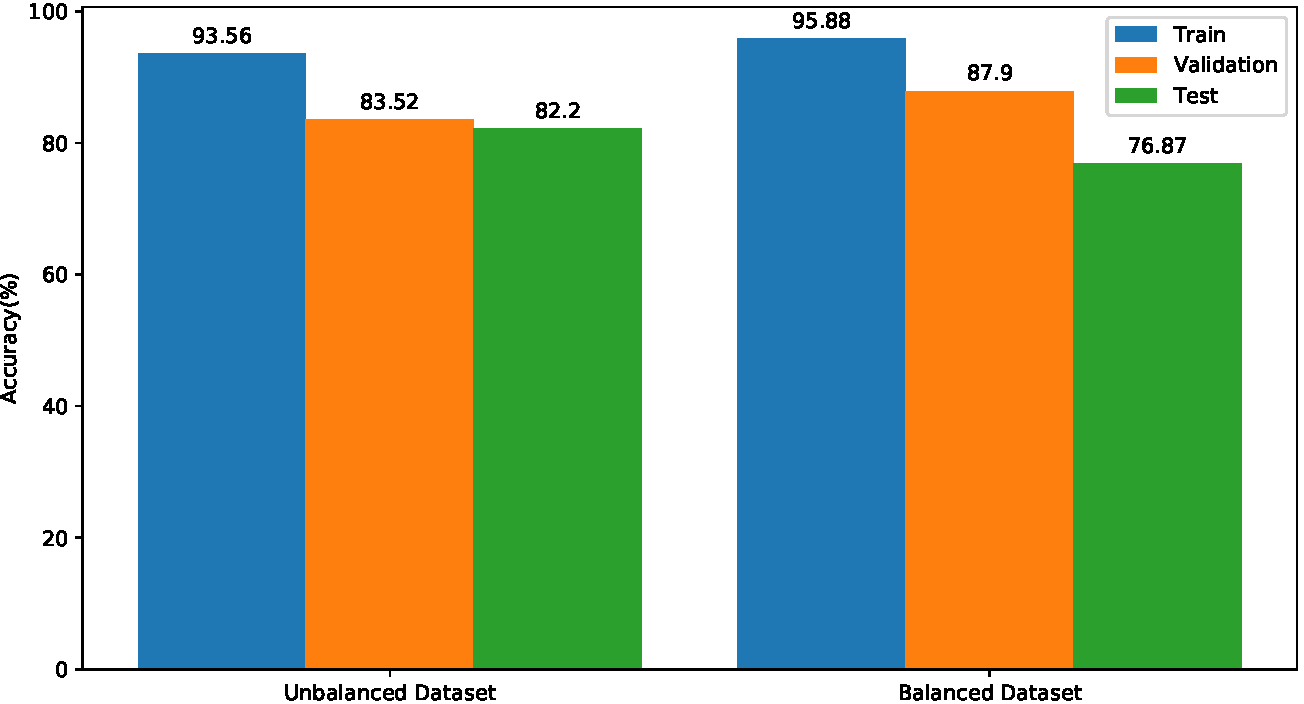
\includegraphics[width=\textwidth]{figs/densenet201_acc_comp.pdf}
        \caption{Comparison of the accuracy of balanced and unbalanced datasets with 20264 samples for the train, validation and test sets.}
        \label{fig:densenet201_acc_comp}
    \end{figure}
    
    Considering the results from figure \ref{fig:densenet201_balanced_samples_metrics_comp} it seems that increasing the dataset through augmentation does improve BMA on the test set to a certain set size, specifically around 40000 samples. Past that point, while the accuracy keeps improving the BMA does not change significantly. These results show that past 40000 samples the improvements come from the overepresented classes that were undersampled and are now getting better performance significantly improving accuracy. It is also important to notice how the BMA metric aproximates the accuracy metric when the datasets are balanced, which is the case of the validation and train sets, but in the test set they diverge as the test set is not balanced. Another important consideration is that between 20000 and 30000 samples, there is breakeven point between validation and train BMA and accuracy as the validation set starts attaining better performance than the train set. That breakeven point happens when the number of synthetic samples is superior to the number of original samples on the train and validation sets  \par
    
    \begin{figure}[ht]
        \centering
        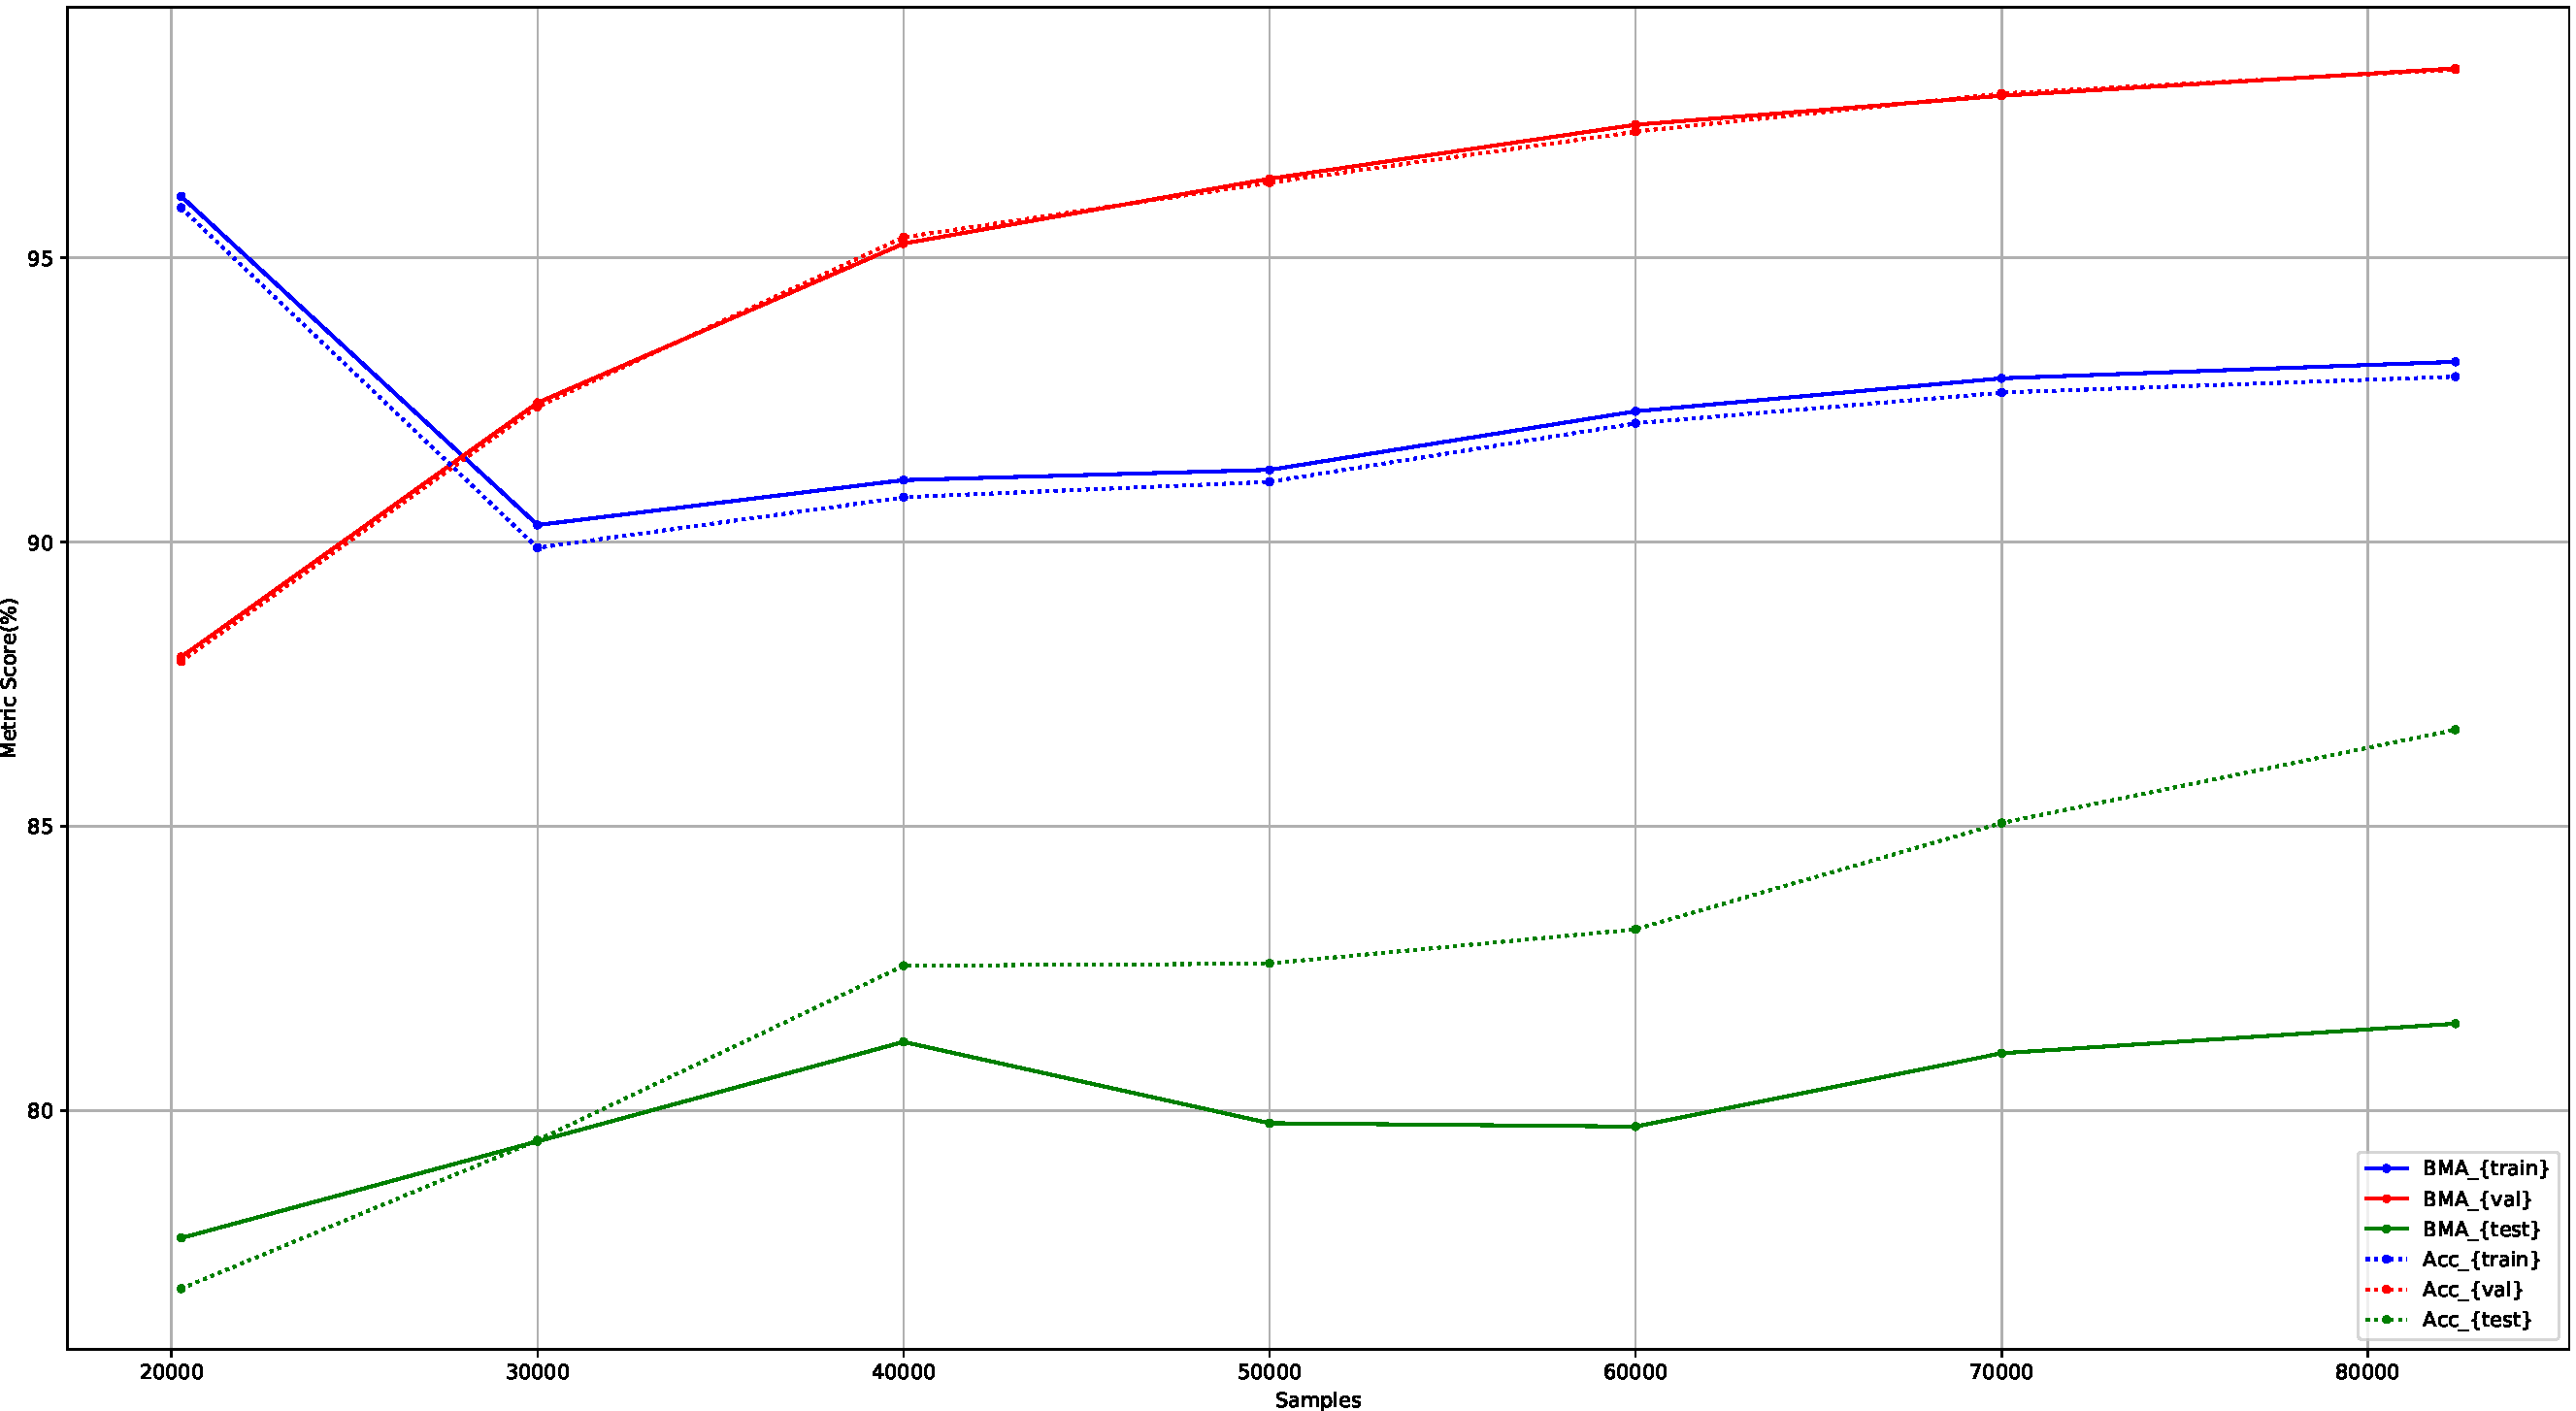
\includegraphics[width=\textwidth]{figs/densenet201_balanced_samples_metrics_comp.pdf}
        \caption{Comparison of the balanced multi-class accuracy for different balanced dataset sizes using the described oversampling and undersampling techniques}
        \label{fig:densenet201_balanced_samples_metrics_comp}
    \end{figure}

    Finally, the results on the test set show the remarkable impact of data augmentation used as a class balance measure, with a accuracy of $86,14\%$ and a balanced multi-class accuracy of $80,9\%$, which is a quite significant improvement from the fine-tuned model trained at \autoref{section:hyperparameters}. Presumably, this jump in performance is due to an increase in sample size for classes that are underrepresented on the original dataset. We can confirm such hypothesis by looking at Figure \ref{fig:82400_balanced_conf_matrix}, which in comparison with Figure \ref{fig:hyperparameter_tuned_conf_matrix} shows that the network is much more capable of classifying correctly underrepresented classes. \par
    \begin{figure}[ht]
        \centering
        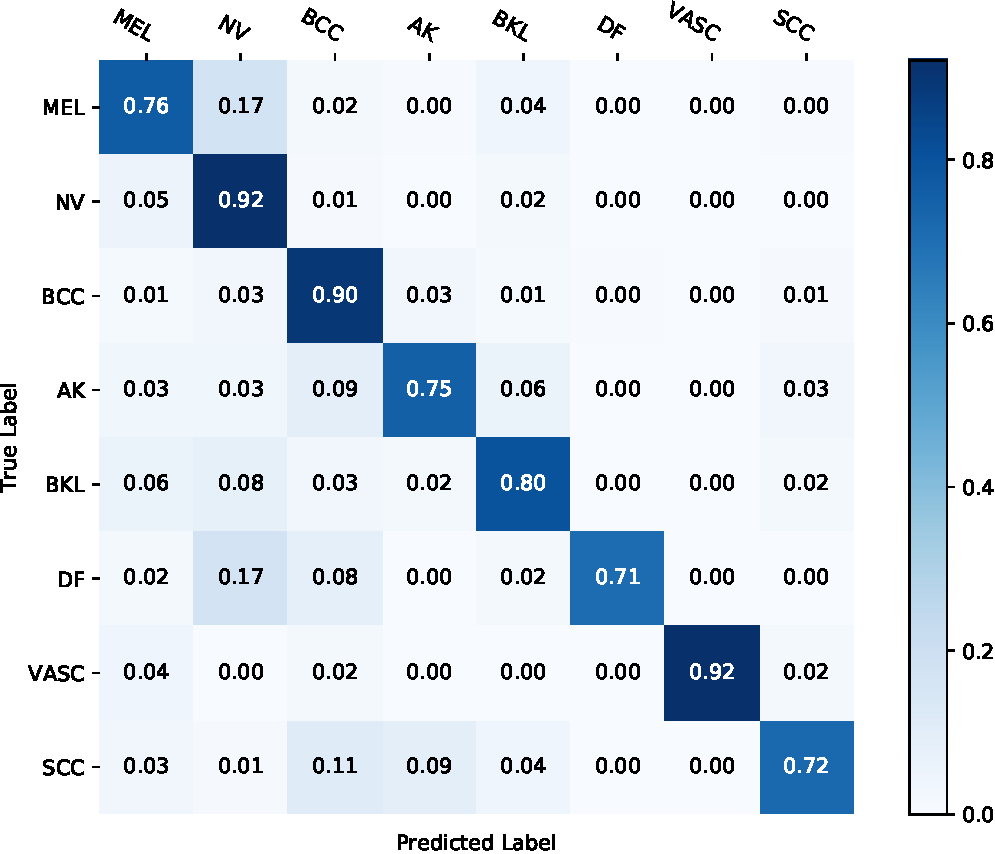
\includegraphics[width=0.6\textwidth]{figs/densenet201_82400_balanced_conf_matrix.pdf}
        \caption{Confusion matrix of hyperparameter tuned DenseNet201 trained with 82400 balanced samples}
        \label{fig:82400_balanced_conf_matrix}
    \end{figure}
    
    
\section{Model ensemble} \label{section:ensemble}
    The literature suggests that the most successful approaches towards ISIC challenges are those based on ensemble of classifiers \cite{humanvsisic2018}. Often these classifiers have model and hyperparameter variations between each other, and are combined through either a weighted or unweighted softmax probability averaging scheme. Other approaches like voting schemes can also be used but those do not take into account the relative certainty of the model predictions. On that account, based on Figure \ref{fig:pre_trained_model_val_comp}, several models \par
    
    One important aspect to consider is how to produce meaningful variations between each model. By simply picking variations within a model architecture not enough variation is produced because often smaller models are just scaled versions of a baseline model, which means that averaging such models would not significantly increase the overall performance. Such is the case of models like VGG16 and VGG19 or EfficienNetB2 and EfficientNetB0. As such, to filter combinations of models the best performing model from each architecture in figure \ref{fig:pre_trained_model_val_comp} was chosen, specifically, VGG16, ResNet152, DenseNet201, InceptionResNetV2 and EfficientNetB2. Additionally, for simplification all models will use the hyperparameters optimized for DenseNet201 in section \autoref{section:hyperparameters}, while also using the best data augmentation schema from \autoref{section:balance}. Results are shown in table \ref{tables:82400_ensemble}. \par
    
    \begin{table}[h]
        \centering
        \begin{tabularx}{\textwidth}{|l|X|X|}
            \hline
            Model & Model $BMA$ & Model Accuracy \\ \hline
            VGG16 & $\approx$0.7533 & $\approx$0.824 \\ \hline
            ResNet152 & $\approx$0.797 & $\approx$0.858 \\ \hline
            DenseNet201 & $\approx$0.815 & $\approx$0.867 \\ \hline
            InceptionResNetV2 & $\approx$0.811 & $\approx$0.862 \\ \hline
            EfficientNetB2 & $\approx$0.820 & $\approx$0.851 \\ \hline
            Ensemble of best 2 & $\approx$0.842. & $\approx$0.878 \\ \hline
            Ensemble of best 3 & $\approx$0.846 & $\approx$0.891 \\ \hline
            Ensemble of best 4 & $\approx$0.841 & $\approx$0.894 \\ \hline
            Ensemble of 5 & $\approx$0.836 & $\approx$0.893  \\ \hline
        \end{tabularx}
        \caption{Ensemble comparison}
        \label{tables:82400_ensemble}
    \end{table} 

    Results from Table \ref{tables:82400_ensemble} show significant improvements of all ensembles over single model performance on both balanced multi-class accuracy and accuracy, with the ensemble of 3 being the best performing one reaching near 90\% accuracy. One can observe that more models are not necessarily better, as the ensemble of the best 4 and the ensemble of 5 yield worse performance than the ensemble of the best 3. This can be attributed to the discrepancy of on the performance of VGG16 and ResNet152 in relation to the rest, which as a consequence of the averaging scheme bring the performance metrics down. However, the models of the ensemble of the best 3 all have similar performance individually, and overall benefit from being ensembled together, which can be attributed to the variation within each model architecture. \par
    
    Finally, the confusion matrix of the ensemble of the best 3 models is shown in Figure \ref{fig:densenet201_best_ensembe_3}. Results show that overall every class has a slightly better performance when compared to the single model performance of DenseNet201 at Figure \ref{fig:82400_balanced_conf_matrix}. \par
    
    \begin{figure}[ht]
        \centering
        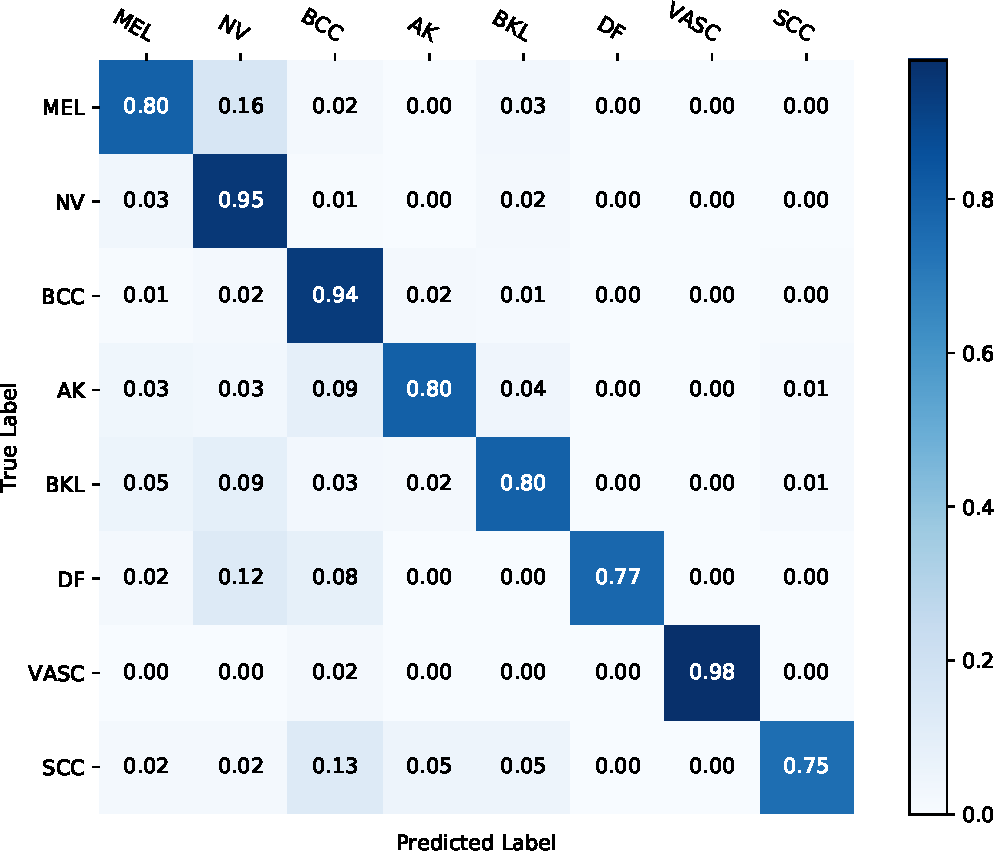
\includegraphics[width=0.6\textwidth]{figs/densenet201_best_ensembe_3.pdf}
        \caption{Confusion matrix of the ensemble of the best 3 pre-trained models (DenseNet201, EfficientNetB2 and InceptionResNetV2). Each model is trained with 82400 balanced samples with the best hyperparameters obtained from \autoref{section:hyperparameters}}
        \label{fig:densenet201_best_ensembe_3}
    \end{figure}



\section{Out of distribution detection} \label{section:outdist}
    The presented models shown that neural nets can be effective predictors to diagnose skin lesions. However, these models remain ignorant to its prediction confidence, (i.e. determining if a sample is or is not part of the training distribution). Although several approaches for dealing with out of distribution samples have been proposed on \autoref{chapter:sota}, we will only explore 3 of them. Namely:
    
    \begin{itemize}
        \item Following Gessert et al's (ISIC 2019 winner) approach, we will train models with an additional outlier class, with additional samples.
        \item Following Zhou et al's submission, we are going to apply a top-1 softmax probability threshold.
        \item Finally, we are going to integrate the ODIN classifier \cite{odin}, following Wang's approach \cite{Wang}.
    \end{itemize}
    
    \subsection{Outlier class}
    
    \subsection{Softmax threshold}
    
    \subsection{ODIN classifier}